\documentclass[12pt]{article}
\usepackage[utf8]{inputenc}
\usepackage[T1]{fontenc}
\usepackage{titlesec}
\usepackage{enumitem}
\usepackage[left=2.54cm,top=3cm,right=2.54cm,bottom=3cm]{geometry}
\usepackage[]{csquotes}
\usepackage[sorting=none]{biblatex}
\usepackage{hyperref}
\usepackage{graphicx}
\usepackage{upgreek}
\usepackage{setspace}
\usepackage{longtable}
\usepackage{eurosym}
\usepackage{rotating}
\usepackage[table]{xcolor}
\usepackage[acronym,toc]{glossaries}

\renewcommand{\arraystretch}{1.3}
\renewcommand{\glsnamefont}[1]{\textbf{#1}}

\graphicspath{ {00images/} }

\addbibresource{mendeley.bib}
\setlength{\parindent}{10ex}

% Acronyms %%%%%%%%
\makeglossaries
\newacronym{dtl}{DTL}{Danish Transport and Logistics}
\newacronym{its}{ITS}{Intelligent Transport Systems}
\newacronym{wave}{WAVE}{Wireless Access in Vehicular Environments}
\newacronym{V2V}{V2V}{Vehicle to Vehicle}
\newacronym{V2I}{V2I}{Vehicle to Infrastructure}
\newacronym{V2X}{V2X}{Vehicle to Everything}
\newacronym{arib}{ARIB}{Association of Radio Industries and Businesses}
\newacronym{sartre}{SARTRE}{Safe Road Trains for the Environment}
\newacronym{VANET}{VANET}{Vehicular Ad-hoc Network}
\newacronym{GPS}{GPS}{Global Positioning System}
\newacronym{LDM}{LDM}{Local Dynamic Map}
\newacronym{OBU}{OBU}{On-board Unit}
\newacronym{RSU}{RSU}{Road-side Unit}
\newacronym{DSRC}{DSRC}{Dedicated Short Range Communication}
\newacronym{ROI}{ROI}{Range of Interest}
\newacronym{FV}{FV}{Following Vehicle}
\newacronym{HMI}{HMI}{Human-machine interface}
\newacronym{IEEE}{IEEE}{Institute of Electrical and Electronics Engineers}
\newacronym{CACC}{CACC}{Cooperative Adaptive Cruise Control}
\newacronym{HDV}{HDV}{Heavy-duty Vehicle}
\newacronym{CC}{CC}{Cruise Control}
\newacronym{LACC}{LACC}{Look-ahead Cruise Control}
\newacronym{CLAC}{CLAC}{Cooperative Look-ahead Cruise Control}
\newacronym{ACC}{ACC}{Adaptive Cruise Control}
\newacronym{CFD}{CFD}{Computational Fluid Dynamics}
\newacronym{ETSI}{ETSI}{European Telecommunication Standards Institute}
\newacronym{PHY}{PHY}{Physical Layer}
\newacronym{MAC}{MAC}{Media Access Control}
\newacronym{DSSS}{DSSS}{Direct Sequence Spread Spectrum}
\newacronym{DPBSK}{DPBSK}{Differential Binary Phase-shift Keying}
\newacronym{CCK}{CCK}{Complementary Code Keying}
\newacronym{DQPSK}{DQPSK}{Differential Quadrature Phase-shift Keying}
\newacronym{DBPSK}{DBPSK}{Differential Binary Phase-shift Keying}
\newacronym{DIFS}{DIFS}{Distributed inter-frame Space}
\newacronym{SIFS}{SIFS}{Short Inter-frame Space}
\newacronym{CSMA}{CSMA/CA}{Carrier Sense Multiple Access with Collision Avoidance}
\newacronym{DCF}{DCF}{Distributed Coordination Function}
\newacronym{EIFS}{EIFS}{Extended Inter-frame Space}
\newacronym{CW}{CW}{Connection Window}
\newacronym{RTS}{RTS/CTS}{Request To Send / Clear To Send}
\newacronym{OFDM}{OFDM}{Orthogonal frequency-division Multiplexing}
\newacronym{QAM}{QAM}{Quadrature Amplitude Modulation}
\newacronym{QPSK}{QPSK}{Quadrature Phase-shift Keying}
\newacronym{BPSK}{BPSK}{Binary Phase-shift keying}
\newacronym{EDCA}{EDCA}{Enhanced Distributed Channel Access}
\newacronym{AC}{AC}{Access Class}
\newacronym{AIFS}{AIFS}{Arbitration Inter-frame Space}
\newacronym{TDMA}{TDMA}{Time-division Multiple Access}
\newacronym{LTE}{LTE}{Long Term Evolution (Mobile Communication Standard)}
\newacronym{PMD}{PMD}{Physical Medium Dependent}
\newacronym{PLCP}{PLCP}{Physical Layer Convergence Protocol}
\newacronym{LLC}{LLC}{Logical Link Control}
\newacronym{PDU}{PDU}{Protocol Data Unit}
\newacronym{MPDU}{MPDU}{MAC Protocol Data Unit}
\newacronym{FCS}{FCS}{Frame Check Sequence}
\newacronym{LSDU}{LSDU}{Link Service Data Unit}
\newacronym{DSAP}{DSAP}{Destination Service Access Point}
\newacronym{SAP}{SAP}{Service Access Point}
\newacronym{SSAP}{SSAP}{Source Service Access Point}
\newacronym{SCH}{SCH}{Service Channel}
\newacronym{CCH}{CCH}{Control Channel}
\newacronym{DCC}{DCC}{Decentralised Congestion Control}
\newacronym{WSM}{WSM}{WAVE Short Message}
\newacronym{WSMP}{WSMP}{WAVE Short Message Protocol}
\newacronym{IP}{IP}{Internet Protocol}
\newacronym{PSID}{PSID}{Provide Service Identifier}
\newacronym{QoS}{QoS}{Quality of Service}
% \newacronym{}{}{}
% \newacronym{}{}{}
% \newacronym{}{}{}
% \newacronym{}{}{}


%%%%%%%%%%%%%%%%%%% 

\begin{document}
% 
\tableofcontents
\pagebreak

\begin{singlespacing}
\setglossarystyle{long}
\printglossary[type=\acronymtype, title=List of acronyms and abbreviations, toctitle=List of acronyms and abbreviations, nonumberlist]
\printglossary
\end{singlespacing}

\section{Introduction}
% 
Travelling by car is part of everyday life of millions of people. Over the past decades, the number of vehicles on the roads has only been increasing\footnotemark. This brings up several challenges. How to fight the increasing pollution, to which road traffic contributes to? What to do, when there are so many cars, that they can not fit on existing roads? Some of these problems might be addressed by the concept of \emph{platooning}.\par
% 
\footnotetext{\url{http://www.huffingtonpost.ca/2011/08/23/car-population_n_934291.html}, accessed 20/05/2017}
% 
The term \emph{platooning} has been popularised by the project SARTRE \cite{Chan2012ProjectSARTRE}, conducted between 2009 and 2012, which investigated, how vehicles can drive in groups, closely following each other. There are several benefits of this concept, which include fuel savings (due to drafting\footnotemark), better utilisation of the road (as vehicles in platoon may drive closer to each other), increased safety and comfort for the users, since the drivers of vehicles travelling in the platoon (except the lead vehicle driver) do not need to focus on the road and may rest or work.\par
% 
\footnotetext {Drafting is a technique where two vehicles align, utilising the slipstream of the lead vehicle and thus reducing the air resistance of following vehicles.}
% 
The downside of platooning is increased responsibility of the lead vehicle driver (which may require them to take additional training). Furthermore, the drivers in following vehicles may not be completely aware of road conditions at all times and can fail to take over the control of the vehicle, in case of technological errors or other unforeseen circumstances. Another issue to be addressed is how to motivate the drivers to become the lead vehicle of the platoon, as we will discuss later on, their benefits are lower than those of following vehicles.\par
% 
In order to achieve implementation of this concept in practice, there is number of crucial aspects to be considered, such as:
\begin{itemize}[noitemsep]
    \item \emph{Use-cases of the system} (e.g. How is the system used?)
    \item \emph{Technology} (e.g. How do the vehicles communicate with each other?)
    \item \emph{Road safety} (e.g. What is the optimal distance between vehicles in platoon?)
    \item \emph{Law} (e.g. Does the law permit semi-/autonomous vehicles?)
\end{itemize} \par
% 
There is quite some research being conducted in this area, but it is not discussed very often in public space. Similarly, no major break-through have been announced lately, increasing the discussion about this on a level that would catch interest of general public.\par
% 
Together with our internal motivation, which includes personal interest in the topic, relevance of the topic, in regards to both our education and on-going development of intelligent cars, and availability of resources, we decided to investigate the area further. While we will not cover all of the aspects mentioned above, there are several areas, which we will pinpoint in problem formulation and research further.\par
%
\subsection{Problem Formulation}

Smart cars utilise many different kind of communication technologies and is currently a very popular topic in today's world. Communication technology is a very broad subject regarding smart cars, to narrow and make our project more specific and manageable we use our problem formulation to stay on track.\par
We decided to focus around one functionality, the platooning. Since the project is being done in Denmark, we decided to base the project in Europe. This also helps narrow down whom the stakeholders for us would be better to get in contact with.
Since this is a communication technology project, we will not be considering how law would affect the project, since it would require substantial research. The main research question thus is:
% 
\begin{itemize}
    \item \textbf{How to enable platooning of heavy duty vehicles on highways, using communication technology, in Europe?}
\end{itemize}
% 
We will investigate this subject from the following angles:
\begin{itemize}[nolistsep,noitemsep]
    \item Is the wireless technology ready to enable platooning?
    \item Who are the stakeholders in the platooning scenario?
    \item What requirements do these stakeholders have on the technology used?
\end{itemize}
% 
\paragraph{After notes}\par
This project is intentionally seen as something that cannot currently be implemented, because of limited infrastructure/smart cars, but this will change in the next 30 years, which is when we believe this would be possible.
% 
\subsection{Delimitation}
To stay on the right track while researching the topic, we came up with a set of delimitations. These are the areas we will not be looking into. First of them is law. The law regarding autonomous and self-driving cars is different from country to country and often changes frequently, as the 'smart cars' are being developed. We will suppose, that platooning is allowed by law, just like operation of self-driving vehicles.\par
Another area we will not look into is human-machine interface. To successfully enable platooning, the solution will very likely involve changes in how truck drivers operate the trucks. Separate research could be made investigating, how this should be done. However, it is not the goal of this report.\par
Even first research on the concept indicates, that fuel savings are present, when vehicles platoon. This leads to savings for companies that run the trucks and may also lead to secondary savings (lower road congestion, lower accident-related costs etc.). A proper business model would need to be introduced to allow fast and easy adaptation of the technology. We will not look into the business and economical side of the issue in this report.
% 
\subsection{Structure of the report}
We will look into the concept from the IT communications perspective. After we present the methodology for this project in 
\textit{\hyperref[sec:methodology]{Chapter} \ref{sec:methodology}},
we research some of the most relevant up-to-date literature in 
\textit{\hyperref[sec:literature]{Chapter} \ref{sec:literature}}. 
Then we present analysis of stakeholders influenced by the platooning in 
\textit{\hyperref[sec:stakeholders]{Chapter} \ref{sec:stakeholders}}.
We will gather data in
\textit{\hyperref[sec:data]{Chapter} \ref{sec:data}}
and come up with use cases and requirements of the system in 
\textit{\hyperref[sec:requirements]{Chapter} \ref{sec:requirements}}
. In the following part of the report - in 
\textit{\hyperref[sec:technology]{Chapter} \ref{sec:technology}}
, we will investigate existing technologies, standards and projects. Namely we will look into \emph{V2V communication, ITS-G5, 802.11p} standards and other technologies and systems we may discover. We will analyse the possible solutions in 
\textit{\hyperref[sec:analysis]{Chapter} \ref{sec:analysis}}.
\hyperref[sec:discussion]{\textit{Discussion}} and \hyperref[sec:conclusion]{\textit{Conclusion}} will follow.
% 
% 


\pagebreak

\section{Methodology}\label{sec:methodology}
% 
In this chapter, we will describe the methods used to find information and get a better understanding of the underlying problems, to be able to provide a potential solution to the problem formulation. This was done by researching similar projects and through their findings we learned what their problems were and how they managed to overcome them. Knowing how some of the parts was put together we were able to make a stakeholder analysis to figure out whom to interview and get an even better understanding of the whole system. Based on this information we created use cases and requirements. Knowing the requirements, we were able to look deeper into specific technologies and with some Empirical data, we could create a potential solution for the project. 
% 
\subsection{Similar projects/Literature review}
First we went through project that specifically had something to do with platooning, and how they were connected, with projects such as Sartre \cite{Chan2012ProjectSARTRE} and Companion \cite{2016CompanionProject}. But to get a better understanding on how the communication behind it works, we needed to branch out to projects, less related but still related regarding to communication technology like SAFESPOT \cite{Safespot} and number of other smaller journal articles, reports and conference proceedings regarding technologies. This gave us a better understanding on what was required for a system like platooning to work.
% 
\subsection{Stakeholder analysis}
When creating a system, many parties is involved both directly and indirectly. To get a better overview of whom gets affected and whom you should listen and take advice from a stakeholder analysis is necessary. This was used to conduct interview with the parties that the analysis suggested. 
% 
\subsection{Interview}
Using the stakeholder analysis, we could figure out who to get in contact with, to get a better understanding of the problems from their point of view. We emailed Car 2 Car Communication Consortium, Scania, Vejdirektoratet (Danish road authority) and Dansk Transport og Logistic (Danish transport organization for drivers) asking for a representative we could interview.
Unfortunately, only DTL responded and accepted our interview, but since the representative was located in Jutland, we decided to conduct a Skype interview instead. The interview was conducted in a semi-structured way, with basic questions to make sure that the interview was going forward, but leaving the interviewer able to make follow-up questions based on the answers from the interviewee. This showed that some of the problems we expected to happen through research was reconfirmed from the interviewee, but there was also new information and problems we had not taken into consideration.
% 
\subsection{Requirement specification/use case}
After using methods mentioned above and gathering all the results from stakeholders analysis, primary and secondary interviews/surveys and state of the art research we realised that concept of platooning has very large amount of requirements, coming form different angles of the system and different stakeholders. Since this project is mostly focusing on ad hoc platooning and communication technologies implementation, our functional and non-functional requirements are also closely related to the research topic. In Solution proposition and Conclusion we will evaluate if requirements for this project can be met and solutions for implementation are found.
% 
\subsection{Technology Research}
The communication technologies we focused mostly on were the standards, ITS-G5 (Europe), WAVE (USA) and ARIB-T109 (Japan), which are being used for V2V communication and platooning as we speak. Going through the lower layers we understood that both ITS-G5 and WAVE are using 802.11 as their fundament, letting us to leave WAVE out of the picture and see the difference in ITS-G5 and WAVE. This gave us a deep understanding on how the data communication between the communication devices are delivered and how to use this in our advantage.


\pagebreak
%
\section{Literature review}\label{sec:literature}
% 
% Introduction to literature review
% 
We can overall conclude that concept of platooning is a heavily researched area. The articles regarding vehicles driving in strings range as back as the eighties \cite{Peppard1974StringSystems}.
Since then the research has been divided into two major areas, as described by \cite{Vinel2015Vehicle-to-vehicleScenarios}. First area is the \emph{Cooperative adaptive cruise control} and the second one is \emph{platooning}. While both touch the scope of our project and should be researched, we focused mainly on the latter.\par
% 
In this chapter we review some of the most recent and most significant works. Two of them are SARTRE \cite{Chan2012ProjectSARTRE} and Safespot \cite{Safespot}, both supported by the European Commission. They chapter continues by discussing the inter-vehicular connectivity and Companion \cite{2016CompanionProject} project afterwards.\par
% 
At the end of the chapter, examples of other works are shown, to describe some of the challenges researched in connection with Platooning.

\subsection{\textit{SARTRE}}\label{sec:SARTRE}

% /include SARTRE notes from Michal/
% \par
SARTRE \cite{Chan2012ProjectSARTRE} stands for Safe Road Trains for the Environment and it is a project which is financed by the European Union. The project is already finished, it lasted for 36 months since September 2009. Its goal was to develop a prototype of system that would be able to coordinate road-trains, so called platoons, in a way that only the first car in a platoon must be driven by a driver and all others are just following it without a need of a driver to pay attention on road. Very important for this project was the use of available technologies meaning that the system may be (in theory) implemented straight after finishing the study. Also, it was designed to work on the actual roads without the need of changing the infrastructure.\par
% 
There have been reasons for realisation of such a project. The traffic on roads is heavier every year, meaning that there are more and more cars being driven which raises several problems: pollution, safety, traffic congestion and limited space for increasing the road capacity. These were the main reasons for realisation of SARTRE. \par
% 
As already mentioned, the main goal was to develop system that would be able to handle platooning. The idea is that in the first vehicle (so called lead vehicle - LV) would be a trained driver which is followed by other vehicles (following vehicles - FV) that after joining a platoon become fully autonomous. Therefore, there are three categories of vehicles with which the system would interact: lead, following and other non-platooning vehicles. The reason is that platoons would be driving down the normal highways mixed with normal (non-platooning) traffic. The system must be able to handle this as there may many cases of direct interaction of the platoon with other vehicles (a vehicle interrupting the platoon by breaking in between two cars, etc.). This however, has not been covered deeply by this project, they are just aware that different situations of interaction may occur and that they must be handled.\par
% 
The architecture of the system was not described to details, there has just been diagrams showing how it looked like (Figure \ref{fig:HW_FW}, showing the hardware configuration of the following vehicle, and Figure \ref{fig:HW_LW}, the configuration of leading vehicle). Also, it was not mentioned what kind (brand, model) of hardware has been used.\par
% 
\begin{figure}[t]
    \centering
    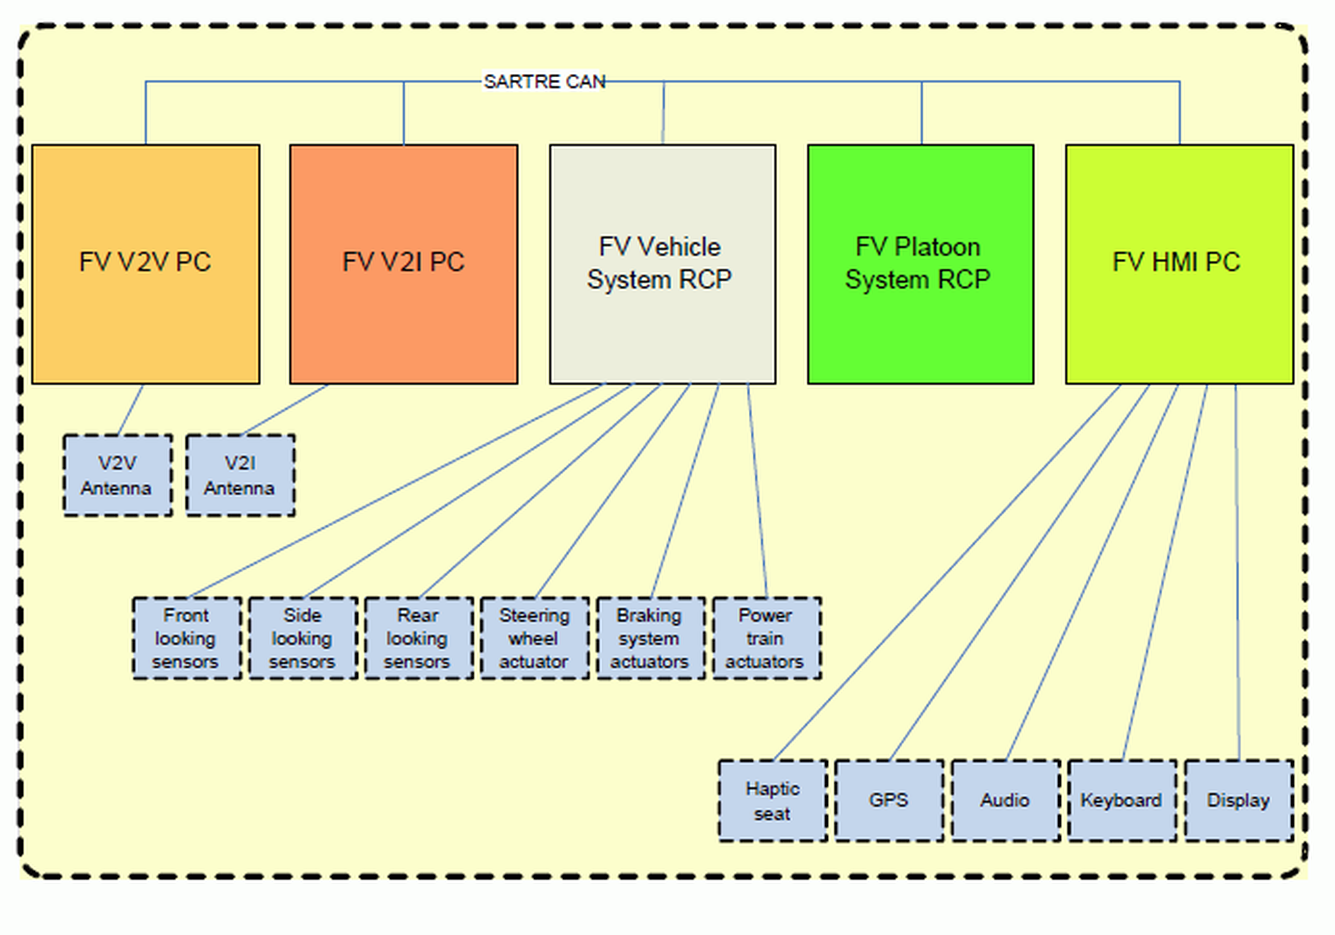
\includegraphics[width=.95\textwidth]{HW_FW}
    \caption{Hardware architecture of following vehicle (vehicle that is platooning). Taken from \cite{Chan2012ProjectSARTRE}.}
    \label{fig:HW_FW}
\end{figure}
% 
\begin{figure}[t]
    \centering
    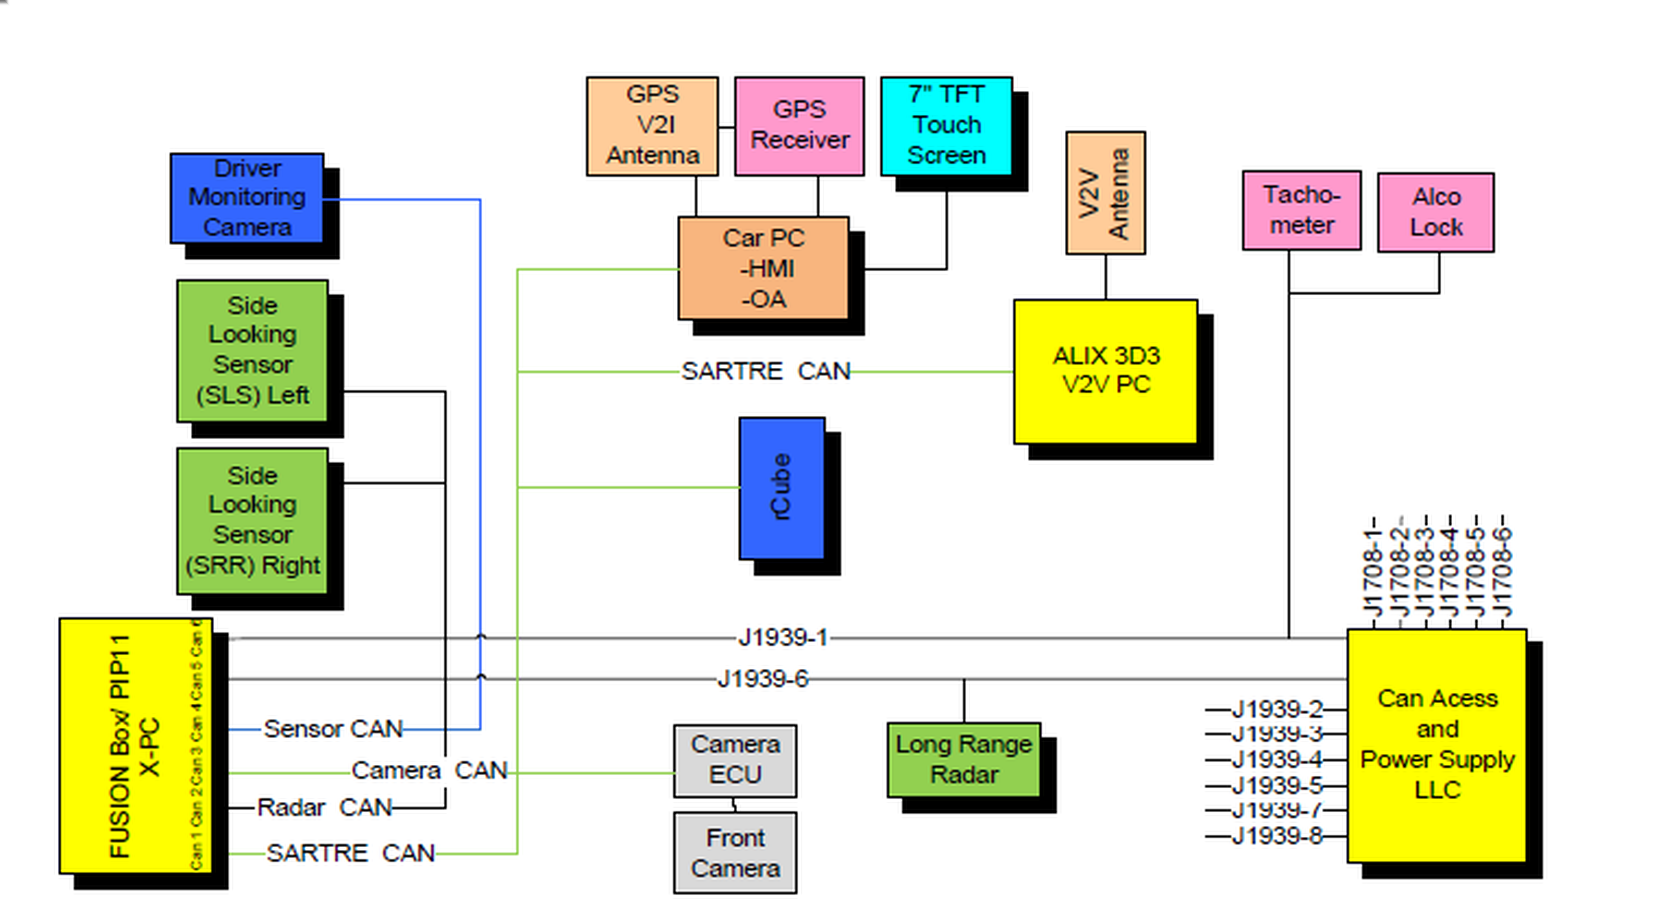
\includegraphics[width=.95\textwidth]{layoutHW}
    \caption{Hardware architecture of the leading vehicle. Taken from \cite{Chan2012ProjectSARTRE}.}
    \label{fig:HW_LW}
\end{figure}
% 
At the end the testing was conducted with truck as the leading vehicle and another truck and three cars as following vehicle. It successfully shown that it is possible to create a platoon of several vehicles where the following vehicles were driven autonomously. Also, that the fuel consumption is being reduced by approximately 10\%.

\subsection{\textit{SAFESPOT}}
In 2006 a project running for 4 years called SAFESPOT \cite{Safespot} was co-funded by the European Commission Information Society and Media, and had an objective to improve road safety. One of the key elements was to have vehicles exchange data between them and with infrastructure (V2V and V2I) to advice or warn the driver of upcoming situation happening.\par
% 
\subsubsection{Architecture}
SAFESPOT is composed of nodes, that communicates with each other through short range wireless communication called VANET (Vehicle Ad-hoc NETwork) using \hyperref[sec:802.11p]{IEEE 802.11p} as physical layer. A node can be in a vehicle or on an infrastructure such as a traffic light. All nodes create data through their sensors or through data from other nodes and are then collected in a multi-layered Database named Local Dynamic Map (LDM).
LDM consist of 4 layers. From bottom up, the first is the static map like Google maps. The second is Landmarks, such as road signs, trees, buildings etc. The third is temporary objects that can change from day to day, such as road work. And lastly Dynamic object which is immediate status, such as congestion, current traffic light colour etc. \cite{Brignolo2008UseProject}.
To locate the position of the vehicles, SAFESPOT uses the road data from GPS, road landmark recognition and dead reckoning\footnotemark.\par
%
% 
\footnotetext{\textquote[Taken from: \url{https://en.wikipedia.org/wiki/Dead_reckoning}]{\textit{In navigation, dead reckoning or dead-reckoning is the process of calculating one's current position by using a previously determined position, or fix, and advancing that position based upon known or estimated speeds over elapsed time and course.}}}
% 
% 
The data rate and communication channel usage is restricted and is one of the physical bottle neck in the system. US WAVE standard (which is similar to SAFESPOT) has a specified data rate of:
\begin{itemize}[noitemsep]
    \item Remote On Board Unit (vehicle): 2320 bit/s
    \item Remote Road Side Unit (traffic light): 22500 bit/s  
\end{itemize}
Though the numbers might be slightly different in Europe, it still shows the bottleneck that exists in this kind of communication channel, especially for On Board Units.\par
% 
Depending on how advanced we want the platooning to be, will lessen the amount of data and how accurate it needs to be. Since SAFESPOT main objective was safety, they needed as many details as possible, to make sure that the driver was given the correct information to avoid a incoming crash. If we want to make platooning only available on highways and only the speed and the brake being controlled, the amount of information needed to be sent to the “VANET” is severely lessened, but if everything were to be automatized, at least as much data as SAFESPOT is needed. The restriction of the data rate is something to take into consideration as well. 

\subsection{\textit{Vehicular Networks}}

% 
Vehicular Ad Hoc Networks (VANETs) are gaining significant amount of interest in educational studies and industry. It is believed that implementation of V2V and V2I communications will lead to success in transportation business in a near future. A report established by Caixing Shao and Supeng Leng from University of Electronic Science and Technology in China \cite{Shao2014AnalysisNetworks} analyses VANET probability in a platoon in a detailed manner.\par
% 
Their V2I solution is tightly coupled with RSU (Road Side Units) implementation on the roads. A problem we are solving in this project is mostly dependant on successful V2V communication and is not meant to be dependant on road infrastructures. With that in mind continuous V2I communication is not necessary for this project, but having some V2I (e.g. in order to facilitate periodical Internet connection) would definitely be beneficial for planning and user experience.\par
% 
Analysis made in University of Electronic Science and Technology in China offers an intelligent solution for continuous Internet access through road side units even if the vehicle is not in the range of RSU. It would use platoon vehicles as relays to reach access to Internet. It is an idea that has potential to be implemented worldwide, so we decided to dig further.\par
% 
Since our platoon solution is not dependant on continuous V2I communication and RSUs are not being implemented in a big scale at the moment \cite{Tonguz2013CarsSolution}, we researched the core idea of using other vehicles in the platoon as relays. Keeping in mind that cars in the platoon will have V2V connection anyways. We have found an interesting report made by students of Carnegie Mellon University in Thailand \emph{Cars as Roadside Units} \cite{Tonguz2013CarsSolution}.\par
% 
Their idea is based on vehicles adopting new wireless communication technology, that is intentionally developed for V2X (Vehicle to everything) - DSRC (Dedicated Short Range Communication) \cite{OfficeoftheAssistantSecretaryforResearchandTechnologyIntelligentSheet}.
Report is proving that implementing RSUs widely might be too costly and inefficient, so they suggest using DSRC enabled vehicles as temporary Road Side Units on a planned briefly stops during the trip. Since the car is acting as RSU for short period of time it would mostly be used to send out messages in case of accident or congestion in ROI (range of interest).

\subsection{\textit{Companion}}\label{sec:Companion}
% 
A very influential research project for platoon implementation in near future, named \emph{Companion} \cite{2016CompanionProject} has been established by SCANIA between 2013 and 2016. Project was coordinated by Magnus Adolfson and involved such automotive giant as Volkswagen.\par
% 
Project's full definition is: \textquote[\footnotemark]{\textit{Cooperative dynamic formation of platoons for safe and energy-optimised goods transportation}} and it is concentrated on research and development of mobility technologies for supervised platooning. Companion's main objective is to improve fuel efficiency and safety of transportation.%
% 
\footnotetext{\url{http://cordis.europa.eu/project/rcn/110628_en.html}, accessed 10/04/2017}%
% 
Problems that are analysed by Companion, are closely related to the ones we are trying to solve with our road train solution in this project and it seems worthwhile investigating work done by experts in the field\footnotemark.\par
% 
\footnotetext{\url{https://youtu.be/_19ui-8f8cw}, accessed 10/04/2017}
% 
Solution suggested by Companion is somewhat new comparing to other platoon projects. They want to form platoons dynamically - meaning vehicle could join and leave platoon whenever it is suitable for that particular vehicle. Participant doesn't have to stay in the platoon for the whole trip, every vehicle can plan different starting and destination locations. Cars would use V2V communication to be able to find nearest platoons and then when in platoon mode, vehicles would communicate constantly to steer, brake and accelerate following vehicles (FV). It is a solution that is not dependant on road infrastructure. Also worth mentioning that project was mostly focused on heavy-duty vehicles.\par
% 
Scope for the project Companion was development and prototype implementation of \emph{Off-Board system for Platoon Coordination} and \emph{On-Board System for Coordinated Vehicle Platooning}.\par
% 
\emph{Off-Board system} will consist of route calculation and optimisation engines and off-board HMI. The system would be controlled by remote dispatchers and is most suitable for planning long distance goods transportation.\par
% 
For developing \emph{On-Board V2V system} interviews with drivers took place. They covered drivers' opinions on vehicle HMIs and platooning in general. Results showed that drivers are positive about new technologies and idea of platooning. Although they would have to build trust of the system for short-distance driving.\par
% 
It is fair to conclude that Companion project was successful in sense that it proved platoon to be high potential and near future technology. Physical and practical tests showed that it could lower fuel consumption up to 12.6\%. Various simulations and driver interviews showed that platooning could drastically improve safety and congestion problems on the roads. Results of various simulations and tests established during Companion project will be analysed more in depth in \hyperref[sec:data]{\textit{Empirical data} section} in this project.
% 

\subsection{\textit{A review of Truck Platooning Projects for Energy Savings}}

This paper \cite{Tsugawa2016ASavings}, published in \emph{Transacions on Intelligent Vehicles}, an IEEE journal, serves as a review of platooning projects that has been done over past decades. Also, it serves as an overview of what platooning is, why there has been projects done since 1950s, what are the objectives of automated platooning and what technologies/projects has been developed since (the most notable once according to authors).
This paper classifies objectives of platooning to three main categories: Energy consumption an CO2 emission, characteristics of the trucking industry and transportation capacity. However, they also realise other positive aspects of it such as safety increase, congestion reduction and comfort.\par
% 
Projects being described in the paper are Automated Trucks in Energy ITS, Electronically Coupled Truck Platoons “KONVOI”, PATH Development of Truck Platooning and CACC Systems. The purpose of each project is being described there along with how it works. Longitudinal controls and system of each project was described there in details as well as its lateral controls and system. The architecture of each system was presented, showing all components of the system and their interaction with each other. For communication between trucks, V2V communication is being used and all of its components are being presented, as well as what information are send/received and what is payload (in some projects, are these information available).\par
% 
The last section of this paper is about impacts of platooning. There are presented findings of the previously mentioned project. Those findings are mostly showing about fuel savings at different gaps between truck.\par
% 
This paper helped us to get better understanding of platooning as it compares several project’s main ideas, aims, technology and findings. Because of that, we were able to get a lot of secondary data for our project, without a need for going through each project separately as all necessary data are presented there.



% Book: Fuel-efficient heavy-duty vehicle platooning
\subsection{\textit{Fuel-efficient heavy-duty vehicle platooning}}
The thesis by Alam A. \cite{Alam2014Fuel-efficientPlatooning}, which was later published also as a book poses as a very valuable resource for this project. The author recognises the growing need of solving the road congestion problem and the persistent need of fuel savings. In the thesis author investigates how the platoons, formed of HDVs (Heavy duty vehicles), can be designed, implemented and what the parameters for optimal fuel savings, while maintaining reasonable level of safety, are.\par
% 
% 
The experiments have been performed with a platoon of three similar HDVs, with 90km long test runs on a highway in Sweden. Fuel consumption was being measured, first, while vehicles were driving alone, and later, while driving in platoon. The test runs were conducted multiple times over period of 5 days to rule out the influences of weather and other variables. The findings show that fuel reduction between 3.9\% and 6.5\% can be obtained for vehicles in the platoon, depending on the weight of the vehicles. Another major influence on the fuel savings is the road gradient. The test runs showed, that with greater road gradient the efficiency of the platoon drops. Reasons for this is the limited engine power and other system dynamics that have not been accounted for, such as gear changes. The thesis also concludes, that it is possible to operate a platoon with inter-vehicular distances between 1-2 meters while maintaining safe operation. Smaller distances could be possibly achieved with more powerful breaks and shorter delays in communication. Furthermore, due to the lack of detailed research, it is concluded that \textquote[\cite{Alam2014Fuel-efficientPlatooning}]{It is still unclear how the unmodeled nonlinearities, such as gear changes, brake dynamics, engine dynamics, and a varying road topography affect the control performance in practice.}
\par
% 
Two models are investigated for controlling the behaviour of the platoon. First, \emph{decentralised} model investigates how the platoon could work, if there is no central control node, but rather each vehicle only communicates with the vehicles surrounding it. The second, \emph{look-ahead control} model describes, how to account for differences among vehicle mass and engine power, which become critical for efficient operation of a platoon in steep road sections, by adjusting the speed of a vehicle prior to approaching a steep road segment.
\par
% 
Technology-wise, the thesis is not very detailed. It states, the the test vehicles are equipped with wireless control unit, which uses IEEE 802.11p standard for communication. Furthermore, GPS and a \enquote{standard doppler radar}. We will further investigate the use of these technologies.
% 
% 
%
% IEEE journal article: Cooperative look-ahead control for fuel-efficient and safe heavy-duty vehicle platooning
\subsection{\textit{Cooperative look-ahead control for fuel-efficient and safe heavy-duty vehicle platooning}}
% 
This article \cite{Turri2016CooperativePlatooning} published in IEEE journal, similarly as \cite{Alam2014Fuel-efficientPlatooning}, considering only HDVs as members of the platoon, investigates how slopes influence the effectiveness of the platoon. It further investigates models that could be used to increase the fuel efficiency of the platoons in hilly areas.
\par
% 
It compares the three approaches to driving vehicles in a group: \emph{Cruise Control} (CC), \emph{Look-ahead cruise control} (LACC) and \emph{Cooperative look-ahead cruise control} (CLAC), each with different rules regarding the control of vehicles' speed. The CLAC is considered as most effective method, as it provides all members of the platoon with sufficient information about road ahead, so they can adjust their own speed accordingly. The CLAC introduces new layer into the platooning, denoted as \emph{platoon coordinator} layer. Such layer \textquote[\cite{Turri2016CooperativePlatooning}]{is responsible  for  the  coordination  of  the  platoon  by  defining a speed profile that is feasible and fuel-efficient for the entire platoon  by  exploiting  preview  topography  information}.
\par
% 
% 
% 
% Vehicle Platoon Formation Using Interpolating Control (article) from AAU
\subsection{Other works}
% 
Number of works, like \cite{Alvarez1997SafeSystems}, \cite{Nowakowski2015CooperativeAlternatives} focus on the system from higher perspectives and discuss, what the overall goal of the system is, what in involves, how it should be used to ensure safety of the traffic and what the architecture of such system should be. Some of the works \cite{Larsson2015TheHeuristics}
approach the problem of platooning from the perspective of mathematics and algorithmization. They try to answer the questions of ideal vehicle routing on (inter-)national scale, in order to optimise the flow of the vehicles and create best strategies for formation of the platoons.
Another important aspect for the problem is how to maximise the fuel savings. Journal article \cite{Turri2016CooperativePlatooning} investigates the changes in the fuel savings in hilly terrain and how to optimise the algorithms of platooning vehicles (trucks) in areas, where they have to break and accelerate often.\par
% 
\subsubsection{\textit{Vehicle Platoon formation}}
The article \cite{Tuchner2015VehicleControl} shows how it is possible to solve the problem of platooning through regulating the vehicles speed and spacing between them with the use of math and algorithms. 3 different solution is being compared with Interpolation Control, Improved Interpolation Control and Model Predictive Control. The differences in result can be found in the article.\par
%No idea how the math works, but at least we can reference to this, when talking about that its not only data between the vehicles, but also alot of math running in the background. 
% 

\subsection{Conclusion}
% Write summary of literature review
The key findings in this chapter, besides the fact that there is a lot of research material about the subject, are:
\begin{itemize}[noitemsep]
    \item There are systems developed, where Cooperative adaptive cruise control (crucial part of platooning) have been successfully tried out and tested. Most of the vehicles used GPS, some kind of wireless communication and a radar to determine distance from vehicles in front.
    \item There are fuel savings while platooning for all vehicles - both leading and following vehicles. These savings depend on distance of the vehicles and slope of the road. The first vehicle has increased consumption than when travelling alone.
    \item Different models can be used for controlling the operation of the platoon, from the perspective of fuel savings and usability (how vehicles join platoons, how two platoons can merge).
\end{itemize}
% 
We have reviewed some of the most significant works concerning platooning, including comprehensive EU-founded projects like SARTRE or Companion. As the research progressed, we kept finding more and more material of great informational value, ranging from detailed technical challenges of the standards used in vehicular environments to broader aspects of platooning. Naturally, not all of them can be listed in this chapter and/or reviewed in great detail. Material listed here, however gives a good picture of the state of the art within the field up to date. Our focus for the next part of this report will be put on determining the stakeholders and their requirements for the platooning concept.\par

\pagebreak

\section{Stakeholder analysis}\label{sec:stakeholders}

\begin{center}
\textquote[\footnotemark]{\textit{A stakeholder is a party that has an interest in a company, and can either affect or be affected by the business.}}
\end{center}
% 
\footnotetext{\url{http://www.investopedia.com/terms/s/stakeholder.asp}, accessed 09-05-2017}
% 
When starting (having) a business, it is important to analyse who your stakeholders are. It is because they may have an affect on your business in one way or another. In the field of platooning we have defined several of them. It starts with truck manufacturers as developers, continues with shippers (companies whose goods is being shipped), carriers (companies that are shipping goods) and truck drivers as users and then government and regulators. Citizens/other drivers are also affected by platooning as it has impact on traffic as whole. Each of them have different power and interest in the platooning and therefore they have been put in the chart below (Figure \ref{fig:stakeholder-chart}).\par
% 
\begin{figure}[h]
    \centering
    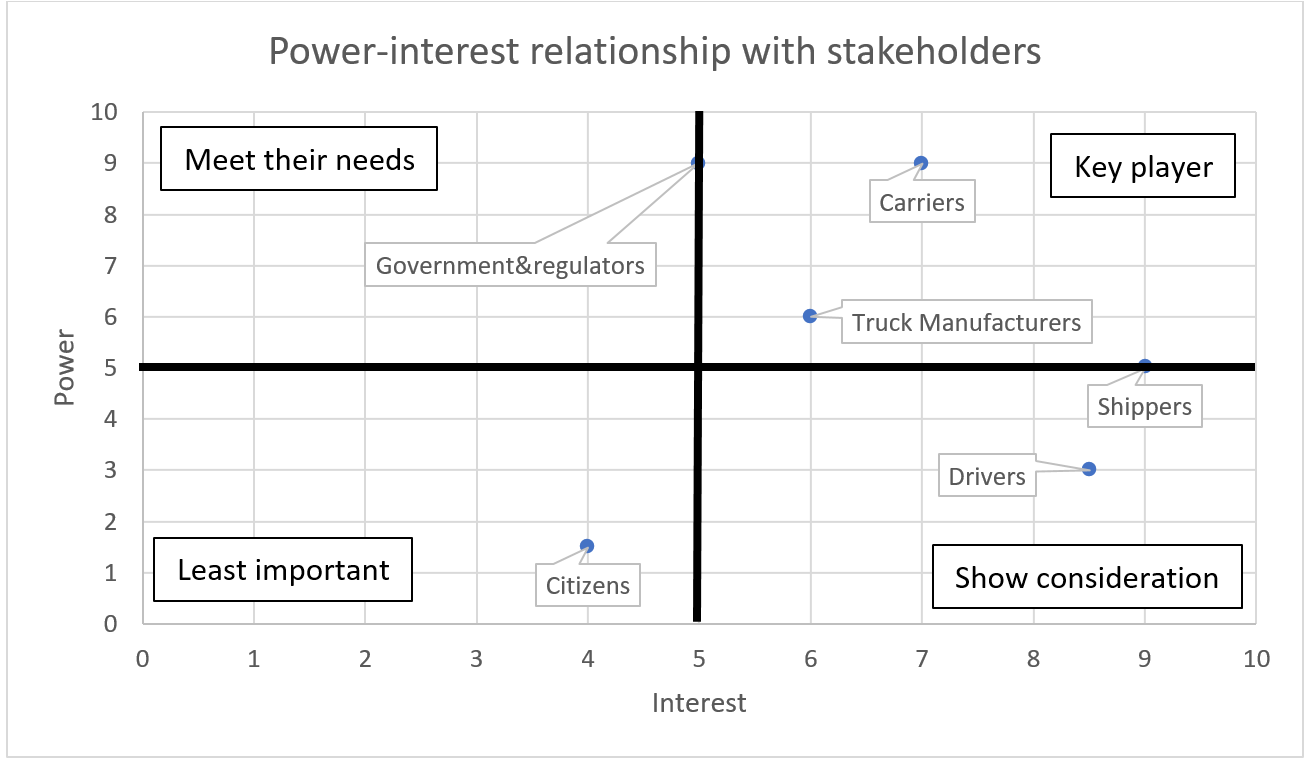
\includegraphics[width=.95\textwidth]{stakeholder-chart}
    \caption{Approximate placement of the stakeholders on the power-interest chart.}
    \label{fig:stakeholder-chart}
\end{figure}
% 
As it can be seen in Figure \ref{fig:stakeholder-chart}, there are different entities with different views. That may cause difficulties in fulfilling needs of all of them as they may be many times in opposition. In following sections we will break it down and look at every stakeholders’ needs separately.\par
% 
\subsection{Shippers}
Are companies/customers that would like to transport goods from point A to B. They are not direct users of platooning and will not have any extra costs because of platooning technology implementation. They only can save money. This may eventually create the pressure from shippers on carrier companies to use the technology, because everyone in the business wants to lower its cost if possible. Therefore, they have kind of big power to force development of platooning and may “force” carriers to adapt the technology.
% 
% 
\par \textbf{Main motivation:} Save money for the transport of products, reducing the risk of products being damaged in crash and building ECO image of the brand by utilising "greener means of transport" (see \hyperref[sec:data]{Chapter} \ref{sec:data} for details on fuel savings).
%
\par \textbf{Biggest obstacle:} Trust in technology has to be established.
% 
% 
\subsection{Carriers}
Companies that are transporting goods. They are the ones bearing the additional costs of trucks (technology) and so they will have a big influence in adapting the technology and its future success. It is up to them to adapt the technology (unless there is a law) and cooperate with each other. This may cause problem between competing companies in the business as they may refuse to share/establish a platoon (this is only supposition). Smaller freight companies are more likely to adapt the technology once the critical mass is reached, meaning that the more platooning vehicles are on road, the more likely they will join.
% 
\par \textbf{Main motivation:} Save money on fuel, safety of truck drivers (see \hyperref[sec:data]{Chapter} \ref{sec:data}). Companies adapting this technology first will have the advantage of being the first and "future ready" as well as it may help them in building better image of the company. 
% 
\par \textbf{Biggest obstacle:} Higher initial cost of a truck, cooperation between transport companies. Being first on the market does not necessary mean advantage over competition because if not enough platooning trucks on the road.
% 
\subsection{Truck manufacturers}
Nowadays, in the technically advanced world, new technologies are being developed constantly. There is no doubt that if a company comes up with a new technology and brings it successfully to the market has a big market advantage, because it can offer something that its competitors cannot at that moment. Therefore, big truck companies like Volvo, Scania, etc. are trying to develop their solutions for platooning and are doing technology push to the market and seize the opportunity of being first. They are also taking part in projects like SARTRE \cite{Chan2012ProjectSARTRE} or Companion \cite{2016CompanionProject} which helps them with gathering crucial data for future development. However, this non-cooperative development and being first hunting, leads to the development of systems that are not usually compatible within different brands.\par
% 
\par \textbf{Main motivation:} By introducing the technology first, get a market share and earn more in sales \cite{Banbury1995TheSurvival}.\par
% 
\par \textbf{Biggest obstacle:} Non-existing regulations and no global standard (system architecture) for platooning, resulting in incompatible systems from different manufacturers.\par
% 
\subsection{Drivers}
% 
They are the ones, that will be benefiting from the technology the most as during their drive, they may be resting, eating or do some other work not connected to driving. Therefore, they would be rested, once they take over the control again, which may lead to lower crash rate. On the other hand, freight companies may lower salaries to drivers as they would not be actively working while platooning or they may be assigned additional work to do while on the road. Platooning may also solve the possible future shortage of truck drivers \cite{OMarah2016TruckImagination} because of unmanned trucks in platoon.\par
% 
\par \textbf{Main motivation:} Possibility of rest during a drive and safety \cite[p. 37]{Chan2012ProjectSARTRE}.\par
% 
\par \textbf{Biggest obstacle:} Drivers may be afraid of new technology and having the truck "out of control" \cite{Sadeghian2016CooperativePrototype}. Also, they may be requested to do other tasks while not driving or earn less.\par
% 
\subsection{Government and regulators}
% 
Government and regulatory authorities play a big role in the process of adaptation of the platooning. By passing laws in favour of platooning the government may help to popularise it among people and speed up its entrance on the market (tax-reliefs, etc.) It is also beneficial for the state to have platooning vehicles on roads as this will save money for them too - safer roads and less need of building new/bigger roads. Regulators however, should set regulations strictly enough to have platooning safe, but on the other hand these regulations should not be barriers for platooning.
% 
\par \textbf{Main motivation:} Saving money on infrastructure (building roads) and hospital charges as safety is higher\cite[p. 37]{Chan2012ProjectSARTRE}.
% 
\par \textbf{Biggest obstacle:} Infrastructure (side road units) may need to be built.\par
% 
\subsection{Citizens and other drivers}
% 
Ordinary people is the last and biggest group of stakeholders in our analysis. They do not have big power over platooning but they are affected by it.
% 
\par \textbf{Main motivation:} Possible saving lower prices for products, safety and less congestion (see \hyperref[sec:data]{Chapter} \ref{sec:data}).\par
% 
\par \textbf{Biggest obstacle:} Afraid of autonomous trucks on platoon.\par
% 
\subsection{Conclusion}
After conducting the stakeholder analysis, we identified our stakeholders which are Carriers, Shippers, Government and regulators, truck drivers, truck manufacturers and other people. We also identified the needs of these stakeholder groups their interests and power. This will help us to derive some requirements from this as well as we will know with which stakeholders we should be cooperating with.
\pagebreak

\section{Empirical data}\label{sec:data}
% 
//Intro about section on empirical data = interviews + surveys other people did
% 
\subsection{Interviews}
% 
//Small intro about interview we did and interview guide we developed.
% 
\subsubsection{Interview with Finn Bjerremand}

Early in the process we have contacted Morten Lindbo, press officer of DTL (Danish Transport and Logistics association). He responded with contacts of their technical consultant and test driver - Finn Bjerremand.\par
% 
Interview on 27th of April was taken via Skype call since we were located in different cities.\par
% 
Finn took part in a research project about truck platooning as a test driver. Trucks in platoon were travelling between two cities in Denmark, distance of around 300km.\par
% 
SCANIA trucks were equipped with ACC (Adaptive Cruise Control) that means it was not fully automated platoon. Finn also noticed that experience of driving with ACC in short distance (9-12 meters) platoon was very similar to regular driving. And because truck drivers usually keep very short distance between each other, Finn thinks that truck platooning will make big improvement for safety on the roads. He was excited about user experience for the drivers as platooning will increase comfort and usability.\par
% 
We introduced Finn with our research problem, and asked about his knowledge about forming ad hoc platoons while being on the road. He saw one main problem comparing to platoons that have set route - "who will pay for who?". Finn thinks it will be difficult to make ad hoc platooning beneficial for everyone, as leading car uses much more fuel than others.\par
% 
Platoon in the experiment did not use any V2V communication and was dependant on ACC for longitudinal automation and drivers for steering the wheel. Finn is also aware of fully automated experiments made by VOLVO or SCANIA, he is excited about driving experience where you don't have to do that much and can even take your breaks without stopping. Although Finn thinks that it will take long time until fully automated platooning will be possible not only on highways.\par
% 
It was relaxed and very informal interview. We greatly appreciate time from Finn Bjerremand. Interview has provided us with useful remarks about driving experience in a platoon and some concerns regarding ad hoc platooning.
% 
\subsection{Secondary data}
% 
//Explanation about other empirical data we gathered (like \cite{Shladover2015IndustryPlatooning}), SAFESPOT, COMPANION, etc. and maybe others (presentation Reza gave us on 04/05?).\par
% 
To prove that platooning is not just another technology being developed without a real added value, several projects and researches has been made to obtain the data to prove its benefits (some of them are mentioned in Literature review chapter - \hyperref[sec:SARTRE]{SARTRE}, \hyperref[sec:Companion]{Companion}). As we didn’t have sufficient budget and time to do the whole development of the system and later on to carry out test to get the data, we looked into those projects to find out whether platooning will be beneficial for people. The areas we tried to cover are fuel consumption, drag, latency, and monetising.
% 
\subsubsection{Fuel savings}\label{sec:fuel-savings}
% 
The lower fuel consumption is one of the main benefit of platooning and one of the main reasons why freight companies would adapt this technology. But in order to convince these companies, there must be clear evidence that platooning really saves fuel. In SARTRE \cite{Chan2012ProjectSARTRE} the CFD (Computational Fluid Dynamic) aerodynamic simulations and real life testing have been done to find it out.
%
\subsubsection*{CFD test}
In CFD test 5 vehicles were involved, 2 trucks and 3 cars, the order was leading truck, following truck and 3 following cars. Tests were done with different distance between vehicles starting with 3 meters till 15 meters. Here vehicles were perfectly aligned behind each other. Figure \ref{fig:cx-reduction} shows by how many percent the drag of vehicles has been reduced with different distances between them. It seems like the closer vehicles are, the better as the drag reduction (Cx) is higher. From simulation, the best fuel saving distance is 3-4 meters. However, having vehicles so close to each other causes instabilities and therefore the best distance would be 6-8 meters according to SARTRE project \cite[p. 33]{Chan2012ProjectSARTRE}.\par
% 
\begin{figure}[p]
    \centering
    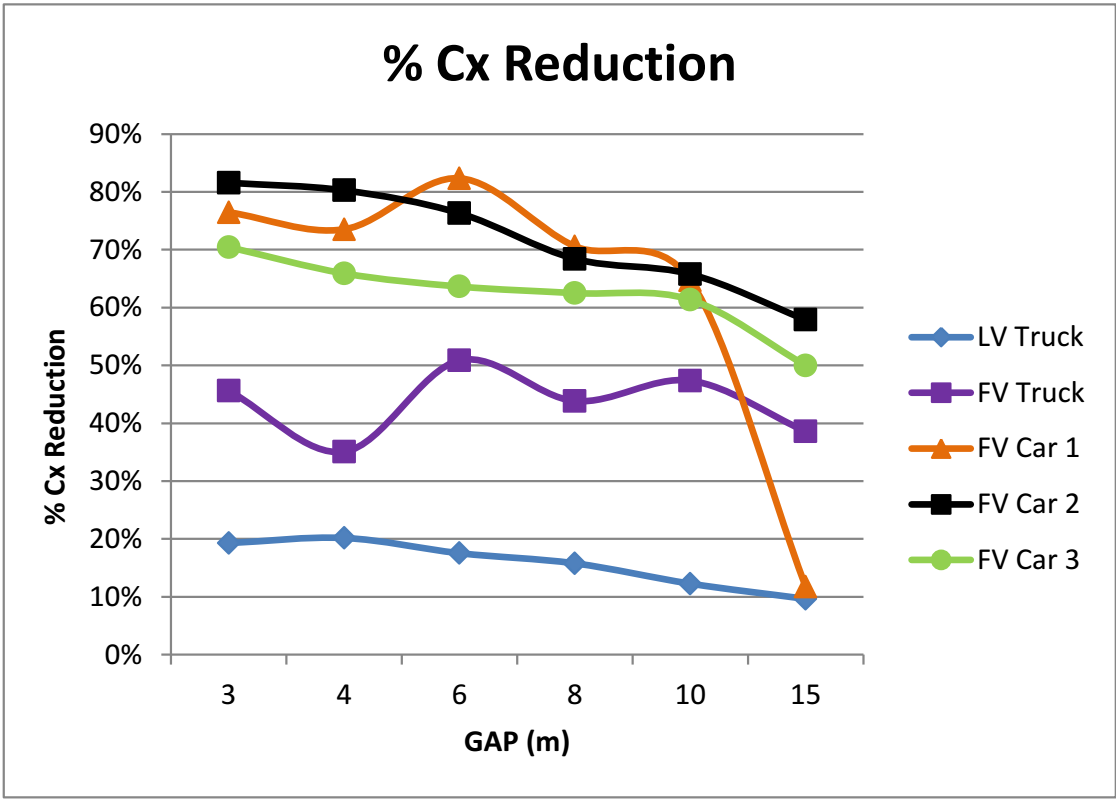
\includegraphics[width=.95\textwidth]{cx-reduction}
    \caption{Drag reduction for platooning vehicles as a function of gap between them. CFD simulation. Taken from \cite{Chan2012ProjectSARTRE}}
    \label{fig:cx-reduction}
\end{figure}
% 
In the test mentioned above the vehicles were perfectly aligned. This however, is very unlikely to happen in real life. Therefore, in the Companion project when making simulation virtually they count with this offset of vehicles and measured difference in drag of 2 truck with different lateral offset, the distance between trucks was 3 meters. The simulated offset was 0.1, 0.25, 0.5 and 1 meter. The Figure \ref{fig:lateral-offset} shows the results of simulations.
% 
\begin{figure}[p]
    \centering
    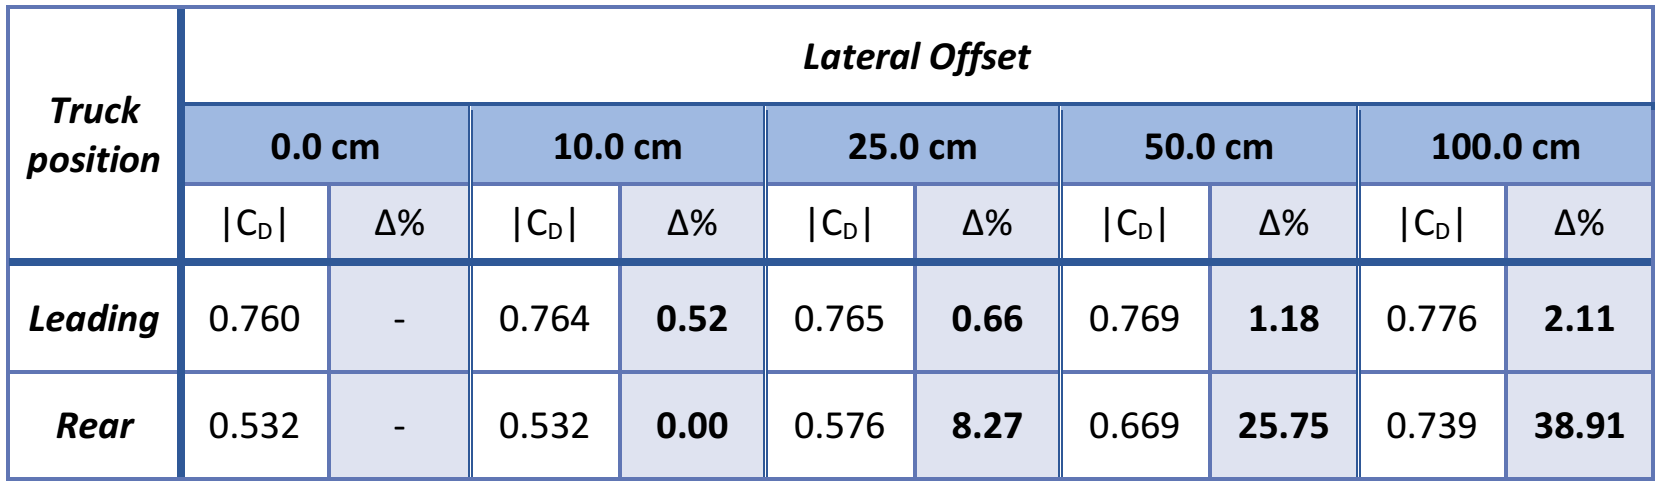
\includegraphics[width=.95\textwidth]{lateral-offset}
    \caption{Difference in drag by lateral offset. CFD simulation. Taken from \cite[p. 19]{Laxhammar2015CooperativeConsumption}}
    \label{fig:lateral-offset}
\end{figure}
% 
As it can be seen in Figure \ref{fig:lateral-offset} small lateral offset of 10 cm does not influence the drag at all, but as the offset is bigger it can be observed that the following truck experiences pretty high values of drag compared to no offset. There is almost 39\% rise in drag when there is 100 cm offset and the drag value of following truck is almost the same as of the leading one. But for leading truck, different offset values did not change much as the maximum drag rise was a bit more than 2\% which is negligible. From this we found that small offset does not have a noticeable impact on the drag but vehicles should be as aligned as possible.\par
%
\begin{figure}[p]
    \centering
    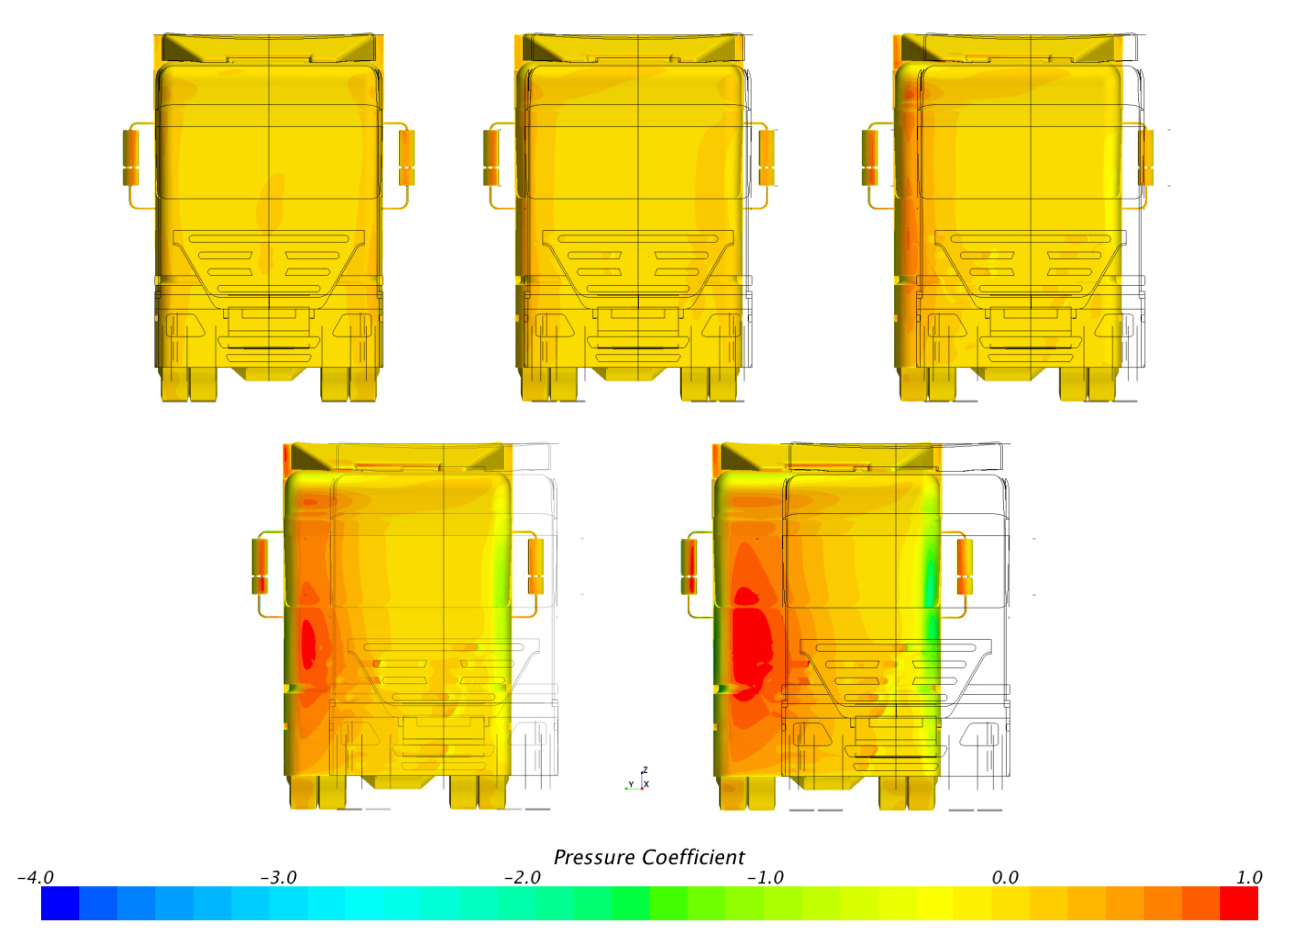
\includegraphics[width=.95\textwidth]{pressure-coef}
    \caption{Pressure on following truck with different offset. CFD simulation. Taken from \cite[p. 19]{Laxhammar2015CooperativeConsumption}}
    \label{fig:pressure-coef}
\end{figure}
% 
% 
\subsubsection*{Real life tests}
In real life tests, a fuel consumption of each vehicle has been first measured separately (not in a platoon) and then in a platoon made up by 2 trucks and 3 cars, the same order as in the CFD simulation. Different distances were tested, starting at 5 meters up to 15 meters. Results are shown in Figure \ref{fig:fuel-savings-full}.\par
% 
As it can be seen in the table, there is a fuel saving effect because of the drag reduction in a platoon in reality as well. The right data could not be measured for cars in distances smaller than 7 meters because of an emergency system which was triggered in cars and made fuel consumption higher. Nonetheless, the graph show that the closer vehicles are the bigger is fuel saving and that also validate that platooning saves fuel.
% 
\begin{figure}[h]
    \centering
    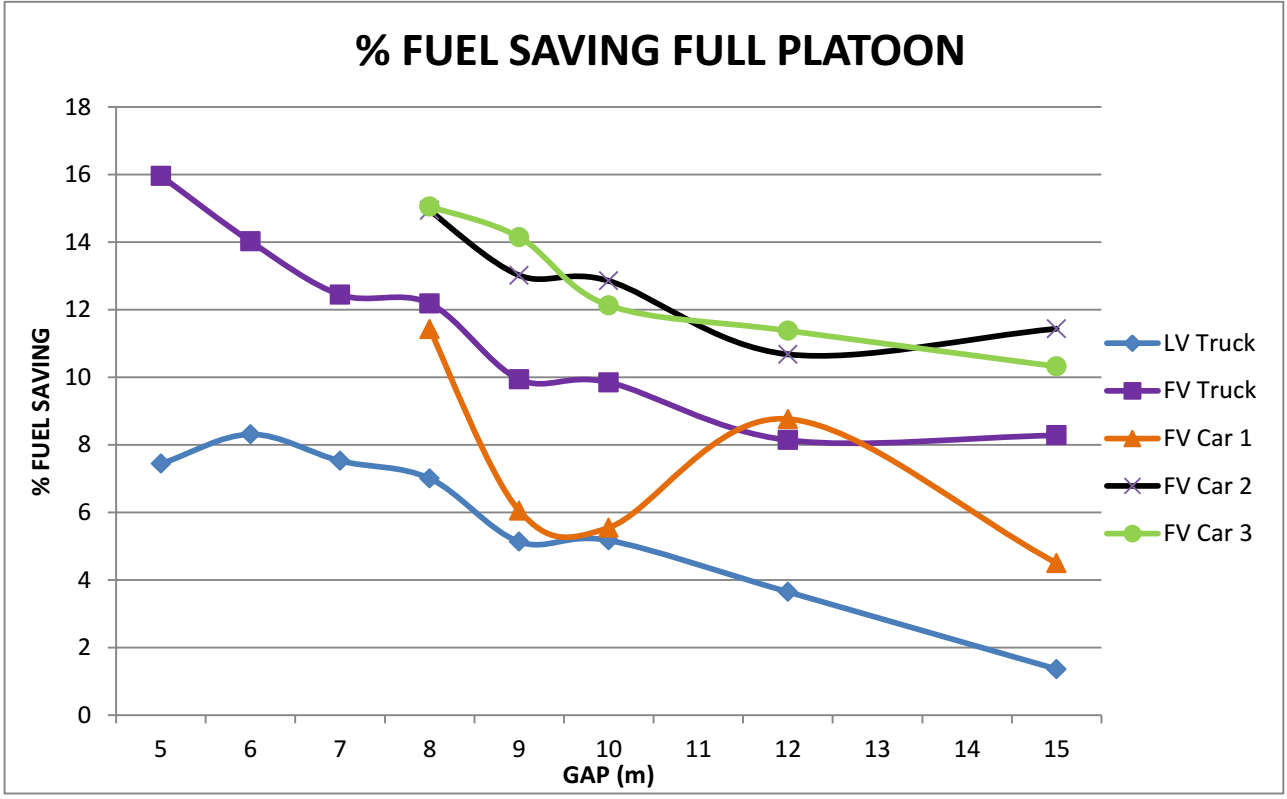
\includegraphics[width=.95\textwidth]{fuel-savings-full}
    \caption{Fuel savings for platooning vehicles. Real-life test. Taken from \cite[p. 36]{Chan2012ProjectSARTRE}.}
    \label{fig:fuel-savings-full}
\end{figure}
% 

% 
\subsubsection{Monetised benefits of platooning}
% 
As shown in the \hyperref[sec:fuel-savings]{previous section}, platooning can save money by lower fuel consumption. But there are higher initial costs and truck will not be platooning 100\% of the time. There comes a question then, whether higher initial costs can be returned over the lifetime of truck and how much can be actually saved. In Companion project, an estimate of the money return has been done, in their deliverable 8.4 \cite{Dr.Hanelt2016CooperativeResults}. To make such a calculation, the estimate price of fuel is needed for year ahead as savings are largely dependent on the price of fuel. Therefore, a forecast for next years had to be done from which the prices will be taken. Table \ref{tab:diesel-costs} shows estimated diesel costs.
% 
\begin{table}[p]
    \centering
    \begin{tabular}{*{10}{|l}| }
        \hline
        \textbf{Year} & 2017 & 2018 & 2019 & 2020 & 2021 & 2022 & 2023 & 2024 & 2025 \\
        \hline
        \textbf{Diesel Price} & 1.18\euro & 1.18\euro & 1.18\euro & 1.20\euro & 1.22\euro & 1.23\euro & 1.25\euro & 1.27\euro & 1.29\euro\\
        \hline
    \end{tabular}
    \caption{Estimated cost of diesel. Taken from \cite[p. 34]{Dr.Hanelt2016CooperativeResults}.}
    \label{tab:diesel-costs}
\end{table}
% 
Other data has been taken also from Companion project deliverable: \textquote[\cite{Dr.Hanelt2016CooperativeResults}]{\textit{The mean age of trucks in Germany is 7.5 years, with 6.2 as the median. Hence, an average use period of seven years per truck is assumed. Relying on previous calculations, a yearly distance of 150,000 km per truck and a fuel consumption of 35 litres per 100 km was assumed. When driving in a platoon of three trucks at a speed of 70 to 80 km/h and a distance of 10 to 20 m between the trucks, the fuel saving potential per truck is 4.99\% on average.}}
Having almost all necessary variables to compute possible investment return, it is needed to choose the commerce year of platooning because of fuel prices. Year 2019 was chosen. Then the last very important think needs to be set and that is the amount of time of which a truck will be platooning, because it will not be doing so always. Four different platooning rates has been chosen: 90\%, 70\%, 50\% and 30\%.\par
% 
\begin{table}[p]
    \centering
    \begin{tabular}{*{3}{|l}|}
        \hline
        \textbf{Platooning rate} & \textbf{Accumulated} & \textbf{Average (p.a.)}\\
        \hline
        \textbf{90\%} & 13,711.72\euro & 1,958.82\euro\\
        \hline
        \textbf{70\%} & 9,186.90\euro & 1,312.41\euro\\
        \hline
        \textbf{50\%} & 4,662.07\euro & 666.01\euro\\
        \hline
        \textbf{30\%} & 137.24\euro & 19.61\euro\\
        \hline
    \end{tabular}
    \caption{Money saved over the lifespan of truck with different platooning rate. Accumulated amount is already lower by initial costs (driving license, truck technology, annual fee, etc.). Accumulated amount is pure saving. Taken from \cite[p.34]{Dr.Hanelt2016CooperativeResults}}
    \label{tab:truck-lifespan}
\end{table}
% 
From the table \ref{tab:truck-lifespan}, it can be seen that even with a low platooning rate of 30\% the higher initial costs will be returned and moreover some small amount of money potentially earned. It is assumed that truck will be platooning more and therefore, this technology should be saving costs to company beside other benefits.
% 
\subsubsection{Latency}
Latency is crucial when it comes to safety in platooning, because if message sent over V2V from leading vehicle to following vehicle fails to arrive on time, it may result in crash. In the SARTRE project (\cite{Chan2012ProjectSARTRE}) they made a test of latency between Back office and Organisation assistant. Back office lies on the server and Organisation assistant is in the vehicle. It communicates with GPS and is sending vehicles’ GPS position to Back office through GSM/UMTS (V2I). Although these are not technologies we are using in V2V it is interesting to see how the latency differs in lower and higher traffic. The test was done on the road in the city as well as outside and in following times: 15:00-16:00 and 18:40–19:30.\par
% 
It can be observed that in the second case, the latency is higher due to the bigger traffic. This reminds us to bear in mind that the bigger the traffic is the bigger the latency and according to that some safety requirements must be set as well (for example: When the latency is higher than X milliseconds, minimum distance between vehicles must be Y meters). Nonetheless the latency should be kept as low as possible, because when using V2V to transmit data the latency may be a difference between safe stop of vehicle and crash.
% 
\begin{figure}[p]
    \centering
    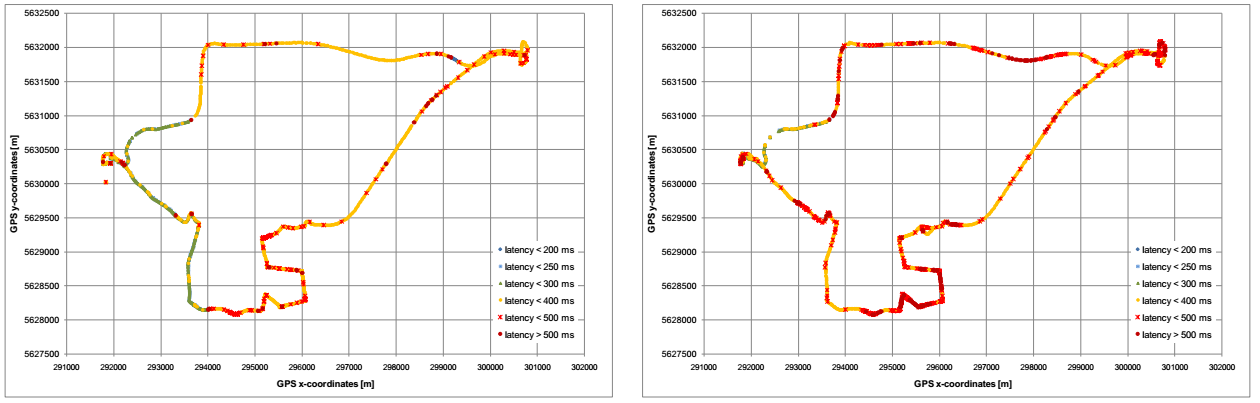
\includegraphics[width=.95\textwidth]{latency}
    \caption{Latency during testing in different day-times: Left 15:00-16:00, right 18:40-19:30. Taken from \cite[p. 24]{Chan2012ProjectSARTRE}}
    \label{fig:latency}
\end{figure}
% 
% 
//Views of Industry on the platooning - little more to be written here.
\pagebreak

\section{Requirement Specification}\label{sec:requirements}
%
In order to satisfy the stakeholders in any technological project, their requirements need to be met. The stakeholders' requirements, however, may sometimes be incomplete, contradictory or unclear. To avoid confusion, requirement specification is often conducted to clear any possible misunderstandings and present a unambiguous set of requirements a system should fulfil. In previous chapter we have identified who the stakeholders are and what their role in the system is. The scope of this report does not allow to analyse all of the requirements possible for the platooning system. Rather we will only focus on technology-related ones. We will list some of the requirements that may influence the decision made while choosing one particular technology. To assist eliciting those requirements, several use cases are presented that represent the most common actions in the platooning scenario.
%
\subsection{Use cases for ad hoc platoon}
% 
There are many different use cases in platooning. It is a very complex and large network made of many moving and fixed parts. It involves V2X communication, where messages are sent and received forth and back at very intense speeds and frequency.\par
%  
This project is mostly focused on technical side of ad hoc platoon implementation and we will only touch upon use cases that are related for this research.
% 
\subsubsection{Find/initiate platoon}
% 
This is initial use case to start using platoon service on the road. Driver using some kind of HMI implementation on his vehicle must be able to detect existing platoon to join or find other drivers that are willing to form a platoon. Long distance communication is required, for driver to be able to plan (slow down, speed up, adjust the route) his entry to platoon. To implement this use case - V2I communication could be used for long-distance implementation and extra functionality, although it must be possible to find or initiate platoon only using V2V. We will discuss technology limitations of V2V and V2I in Empirical data and Technology sections.
% 
\paragraph{Actors of the use case}
\begin{itemize}[noitemsep]
    \item Primary actor - a driver or a vehicle (in a fully automated platoon) which is willing to join/form platoon.
    \item Back-end service - a crucial part for long distance ad hoc platoon planning. It could serve for both business (logistics routing) and personal needs. It should be implemented as a remote server, that would be reached over long distance communication. This back-end solution will keep track of all existing platoons and vehicles that are looking for a platoon. When match is found it will create a route for the user to successfully meet and join the platoon or even several platoons throughout whole distance.
    \item Any other moving or fixed unit on the road (e.g. other cars acting as relays to pass information about existing platoon nearby)
\end{itemize}
% 
\paragraph{Pre-conditions}
\begin{itemize}[noitemsep]
    \item Vehicle that is suitable for platooning - equipped with technologies for V2X communication and fully/semi automated driving.
    \item Access to Internet is also critical for ad hoc platooning, although constant connection might not be necessary, for example when platoon is found and route to it is transferred to vehicle's navigation system, connection could be terminated.
\end{itemize}
% 
\paragraph{Process}
\begin{itemize}[noitemsep]
    \item With help of platoon back-end system user sends a request to find and join platoon. Request should contain details about the trip, like destination, desired travel time, stops and etc. If no platoons are available for desired trip, system would suggest to form a new platoon.
    \item Platoon service could work as spontaneous on-the-go solution, when user decides to join platoon as soon as possible. Or plan ahead option when user submits request for a platoon some time ahead, could be several days or even weeks ahead, and possibly used more by logistic companies or lone truck drivers.
    \item After available platoons are found most important details (route, number of cars and etc) are sent to the user. User can accept or decline the offer.
    \item If user has continuous Internet connection he/she could see live status and location of the platoon, otherwise user would just follow the route, received from platoon back-end. When cars are in the range of direct or relayed V2V communication, status of the platoon would be updated.
\end{itemize}
% 
There are concerns for Internet access implementation in moving vehicles and research is still in ongoing, although even periodical access should be enough for sufficient platoon organisation.\par
% 
\subsubsection{Join/leave moving platoon}
% 
Another crucial use case for platooning concept. This use case is focused around short range communication between vehicles in platoon and the ones who want to join or leave it. Before a vehicle can join/leave moving platoon, all the cars around must adapt and perform necessary actions to make sure safe process. For semi or, in future, fully automated vehicle to successfully join or leave platoon, communication must be precise without any overlapping or interference.\par
% 
\paragraph{Actors of the use case}
\begin{itemize}[noitemsep]
    \item Primary actor - vehicle that is approaching the platoon and ready to join or is in the platoon and wants to leave the platoon because of different routes or any other reasons.
    \item Secondary actors - vehicles around or in the platoon, as well as any available Road Side Unit. While joining/leaving the platoon, V2V or even V2I would make sure that it is safe to perform any actions on the road. For example any RSU or a leading car in the platoon could inform Primary actor that some slow down is ahead, and it is not safe to enter the platoon.
\end{itemize}
% 
\paragraph{Pre-conditions}
\begin{itemize}[noitemsep]
    \item Vehicle has approached platoon in a sufficient distance for V2V communication.
    \item Vehicle has to leave the platoon, for example because it needs to turn into another road or make an unplanned stop.
\end{itemize}
% 
\paragraph{Process}
\begin{itemize}[noitemsep]
    \item Vehicle approaching platoon establishes V2V communication with other vehicles in the platoon. It is up to system design to decide to which and how many cars needs to communicate to join the platoon. For example depending on a car type, or destination, user could be assigned to a different place in the platoon (e.g. front of the platoon, middle or end).
    \item When all conditions for safe join are met, vehicles might need to take some actions to let arriving car into the platoon.
    \item User successfully joins the platoon and stays in it until he/she needs to turn or platoon breaks up for some other reasons.
    \item When user must leave the platoon for any reason other cars will be informed about state change by short distance communication. Same as with joining platoon, any other participant or infrastructure on the road could communicate to the platoon, to make any actions as safe as possible.
    \item Cars in front and back performs necessary actions (e.g. make bigger gaps, slow down and etc.) and Primary actor leaves the platoon.
\end{itemize}
% 
Main concern for the use case is quality and speed of V2V communication. Driving and performing actions in high speed and very short distance between the vehicles might be dangerous, so there cannot be any errors or loss of critical messages during the process.
%
\subsection{Requirements}
After learning about the concept of platooning and establishing state of the art research, we quickly realised that there is a great number of requirements that need to be met for successful real-world platoon implementation. Project this big has a lot of stakeholders, who are very different - platoon gets great attention from governments, logistic companies, truck manufacturers, regular drivers and more. Every stakeholder sees platooning from different perspective and have different requirements for it. While not every user requirement is measured or possible to achieve, it must be considered and evaluated before it gets rejected. And this is only one side of the problem. We have discovered that there are loads of technical requirements as well. Technologies for platooning are still under development and usually there are multiple ways to meet technical requirement and every solution has its pros and cons.\par
Using data from research, primary and secondary interviews/surveys we have gathered and filtered the most relevant requirements following delimitations for this project. Following these requirements we well research possible technical solutions and in the end of project discuss if and how these specifications can be met.\par
%
\subsubsection{General expectations for platooning}
%
\begin{itemize}
    \item\textbf{Platoon must improve safety on the roads} - one of the main reasons for implementing platooning. We learned that humans are not very good drivers, there are thousands of accidents every year in the world, and most of them are caused by human error. In general, automated driving technologies are trying to minimise human mistakes by taking over vehicle's control or assisting drivers on the road.
    %
    \item\textbf{Platooning must lower fuel consumption} - every business is constantly trying to minimise costs and maximise income, in transportation fuel costs are the ones that can be lowered within help of platooning, as Companion project has proven with many different real and simulated tests. Research showed that every stakeholder of platooning expects to lower expenses - whether it's a company that manufactures goods and wants to transport them, or logistics company, or just a simple person using vehicle for travelling. On top of that - lowering fuel consumption means more environment friendly transportation.
    %
    \item\textbf{Improved driving experience} - from interviews and surveys we noticed that drivers who were asked about platooning, firstly think about more comfortable driving. Platoon is aiming to provide better work conditions and efficiency by taking some responsibilities from drivers. Allowing drivers take their breaks while travelling in platoon would not only improve workers satisfaction, but would also save time for the companies.
\end{itemize}
%
\subsubsection{System requirements}
%
System requirements were generated from stakeholders research and our vision for ad hoc platooning. These requirements describe main functions for the system in this project.
%
\begin{itemize}
    %
    \item\textbf{Form platoon as ad hoc network} - this solution is widely discussed in Companion project and is the most important requirement for our project as well. Forming or joining platoon while on the go means that vehicles doesn't have to start their trips from same location and can have different destinations too. It gives opportunity to save costs constantly and for everyone. For example personal car can join platoon of trucks and leave it whenever their routes separates. Trucks will be able to join and leave several platoons throughout their journey.
    %
    \item\textbf{Back-end system must plan long distance trips} - using remote back-end system users will form platoons and plan routes ahead. System must keep track of all platoons that are or will be on the road. This way planned platoons can be combined with users who are willing to join on the go as well as change routes, reform platoons and much more.
    %
    \item\textbf{System must be compatible for both fully and semi automated platoon} - while this is a broad requirement it is self explanatory as well. Until fully automated vehicles take over the roads, some stakeholders will want benefits of platooning using semi automated vehicles. System must be able to adapt to equipment and provide available functionality.
\end{itemize}
%
\subsubsection{Technical requirements}
%
All the research from sections above and user requirements leads us to general technical functional requirements. In this project we mostly focus on communication solutions and requirements listed below has to be met to successfully implement ad hoc platooning.
%
\begin{itemize}
    \item\textbf{V2V must use short-range communication technology} - V2V communication must be implemented with most suitable technology for the case. There are quite few standards around the world, but automated driving is not ready yet for real-world stage and we must evaluate each standards advantages and disadvantages.
    %
    \item\textbf{Connect to backend service over wireless technology} - for planning/finding platoons vehicle must communicate to remote backend service. Vehicle must have at least periodical Internet connection for successful route planning.
    %
    \item\textbf{Join/find platoon without any V2I communication} - if user cannot access Internet to use platoon back-end service, there must be possibility to detect or join platoon using only V2V communication.
    %
    \item\textbf{V2I must allow non-highway platooning} - where V2I communication is available, meaning user has Internet access and road infrastructure is implemented (e.g. traffic lights, any other RSU) platooning must be possible on non-highway roads. 
    %
    \item\textbf{System must be able suitable for different type/brand vehicles} - ad hoc platooning must be available for different brand vehicles. Logistics company might owe different vehicles, so for ad hoc platooning to expand it must be a kind of "cross-platform" solution.
    %
    \item\textbf{Critical messages must reach destination} - critical messages like crash/break warnings must arrive at right order, they cannot be lost or interfered by any other irrelevant communication.
\end{itemize}\par
%
\subsubsection{Conclusion}
Requirements gathered in this chapter reflects main points of our ad hoc platooning project. For real world implementation more specific requirements should be included, which would design the system as a whole. In this case we will investigate technologies necessary to meet listed requirements. In chapter \emph{8. Technology} we will discus our findings and chapter \emph{9. Analysis} we will suggest possible solutions.
\pagebreak

\section{Technology}\label{sec:technology}

Usually, during platooning vehicles are moving with high speeds and therefore can only be connected for a short period of time. Furthermore, due to the high mobility, the neighbouring vehicles may change very often. The connections need to be established locally and with as little set-up time, as possible, otherwise we risk two vehicles being out of range. In this chapter we explore local wireless networks, that are crucial for enabling any platooning scenario. First we see, what \acrshort{VANET} is and what is its relation to Vehicle-to-Vehicle and Vehicle-to-Infrastructure communication. Then we will investigate into the standards that are prevalent in establishing these connections, such as 802.11 or \acrshort{arib} T109. We will cover the basics of the operation of these technologies, as well as their relative performance in platooning scenarios.\par
% 
At the end, we will shortly describe \acrshort{GPS}, as this technology is a requirement in many cases of platooning implementation.

\subsection{Vehicular ad hoc Networks}

\acrshort{VANET} - is a network that combines \acrshort{V2V} (Vehicle-to-vehicle) and \acrshort{V2I} (Vehicle-to-infrastructure) communication.\par
% 
\begin{figure}[ht]
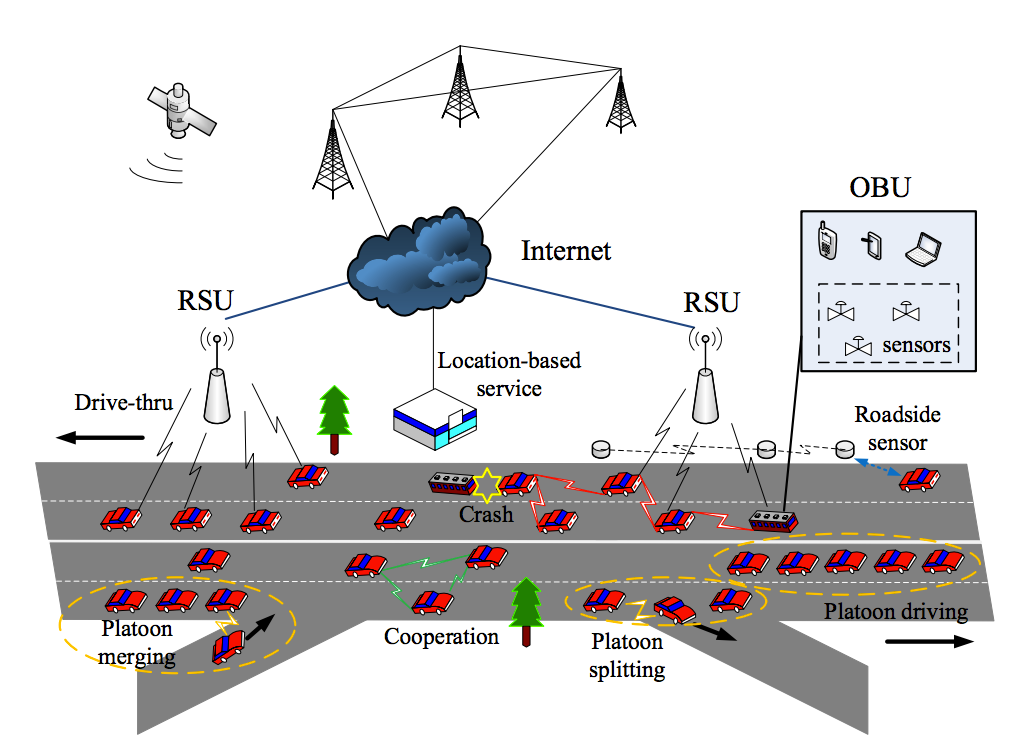
\includegraphics[width=\textwidth]{VANET}
\caption{\acrshort{VANET} formation. In this scenario, all the vehicles are equipped with an \acrshort{OBU} (shown in detail on the right), and can thus communicate with the \acrshort{RSU} and each other. Figure taken from \cite{Jia2016ASystems}.}
% \centering
\label{fig:VANETformation}
\end{figure}
% 
It is large and complex network where vehicles exchange data between each other and any other infrastructure on the road. Traffic participant might receive data, that will prevent accident from happening, relayed from multiple interconnected nodes. Generally \acrshort{VANET}s introduce:

\begin{itemize}[noitemsep,nolistsep]
    \item Safer and more efficient roads
    \item Logistics, transport and service business improvement
    \item Controlled congestion, more comfortable travelling.
\end{itemize}

In Figure \ref{fig:VANETformation} we can see the general architecture of \acrshort{VANET}. One main disadvantage that slows down VANET development that it is dependant on expensive road infrastructure\footnotemark.\par
% 
\footnotetext{\url{http://wifinotes.com/mobile-communication-technologies/what-is-vanet.html}, accessed on 19/04/2017}
% 
\acrshort{VANET} is based on latest mobile communication technologies. Following chapters will discuss present and upcoming technologies that make up the VANET - namely \acrshort{V2V} and \acrshort{V2I}, as these are most relevant for platooning use.


\subsection{V2I}
% 
Vehicle-to-Infrastructure technologies are still under development, but they have great potential. Its main idea is communication with vehicle by any road side unit (e.g. traffic lights, road sensors) to prevent accidents and improve road efficiency.\par
% 
% Vehicle-to-Infrastructure Technologies Expected to offer Benefits
\begin{figure}[h]
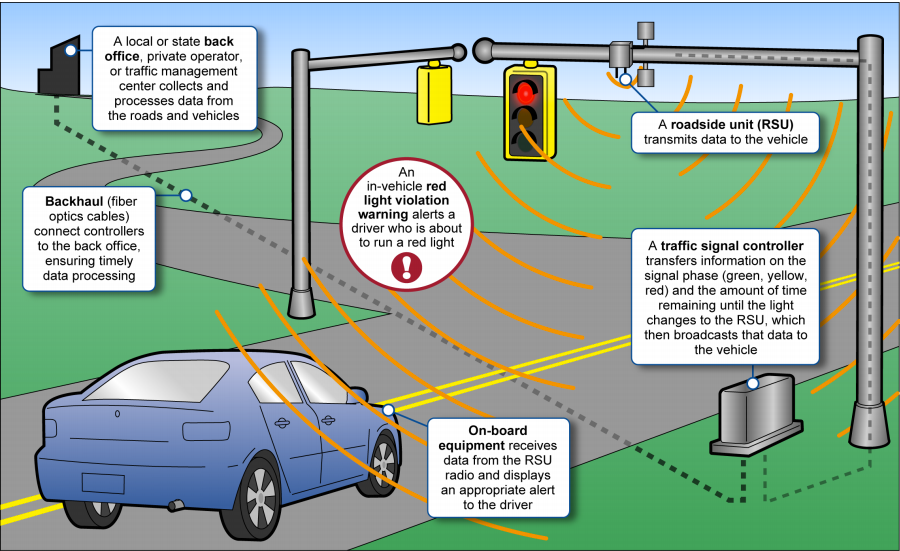
\includegraphics[width=\textwidth]{V2I}
\caption{V21 implementation. Taken from \cite{U.S.GovernmentAccountabilityOffice2015IntelligentExist}.}
\label{fig:V2Iimplementation}
\centering
\end{figure}
% 
There are no standards yet of what V2I system architecture should consist of. Architecture framework defined by USDOTs' ITS Joint Program Office \cite{Dr.Gaspar2014HighlySystems} states, that minimal parts for V2I system are:
\begin{itemize}[noitemsep,nolistsep]
    \item Vehicle On-Board Unit
    \item Roadside Unit
    \item Safe Communication Channel.
\end{itemize}
% 
Communication is based on 802.11p standard by IEEE, which will be discussed in detail in following chapters. A frequency spectrum in 5.9 GHz range was allocated for exact means in U.S. and Europe \cite{2011TheTechnology}. Although, there are some concerns sharing allocated spectrum, since Middle Class Tax Relief and Job Creation Act of 2012 allowed use of 5.9GHz spectrum for any unlicensed devices and that could cause harmful interference for sending and receiving data in V2I communication \cite{U.S.GovernmentAccountabilityOffice2015IntelligentExist}.\par
% 
Despite any concerns, Vehicle-to-Infrastructure is quickly developing and gaining a lot of attention from scientists and businessman worldwide.\par
%
\begin{figure}[h]
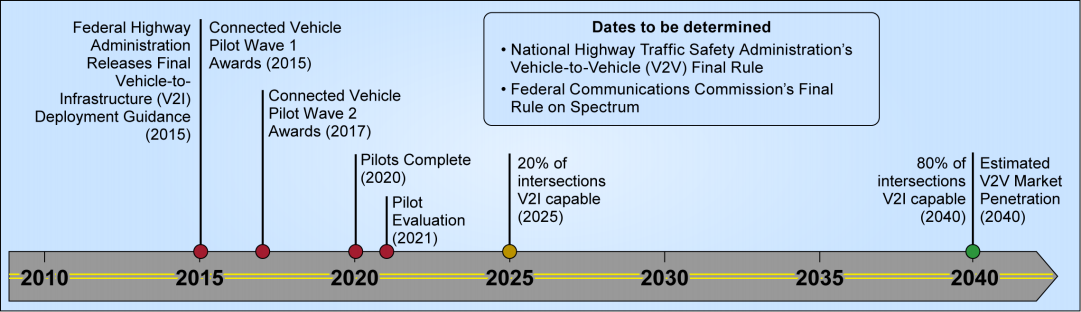
\includegraphics[width=\textwidth]{V2Xtimeline}
\caption{V21 development path. Taken from \cite{U.S.GovernmentAccountabilityOffice2015IntelligentExist}.}
\label{fig:V2Idevelopment}
\centering
\end{figure}


\subsection{V2V}

V2V communication is a vehicle-to-vehicle communication, where vehicles can communicate with each other and share vital information. In last decades, a lot of research (\cite{Chan2012ProjectSARTRE}, \cite{Safespot}, \cite{2016CompanionProject}) has been done in field of V2V, in which different companies, institutions or organisations participated (either as part of project or on their own). This led to creation and adaptation of standards so that developed technologies by different companies can communicate without difficulties. For the short-range communication IEEE 802.11p standard is adopted which is a wireless protocol (similar to Wi-Fi), operating on 5.85-5.925 GHz (depending on country).

\subsubsection{802.11}
% 
When wireless networks first came around, it was expected that the radio medium will only be another physical layer, such as cables. However, it did not take long to see that due to significant differences of radio communication, more detailed, radio-suited standard needs to be developed. In 1991 work has begun in preparation of standard that is today known as \emph{802.11} \cite{Hiertz2010TheUniverse}. The scope of this standard is \textquote[\cite{2016IEEEAccess.}]{\emph{to define one medium access control (MAC) and several physical layer (PHY) specifications for wireless connectivity for fixed, portable, and moving stations within a local area.}}\par
One of the most well-known implementations of 802.11 is Wi-Fi. Naturally, it is not the only one and over the years, several amendments have been accepted to initial standard, to accommodate various needs. As Bilgin\&Gungor \cite{Bilgin2013PerformanceAreas} suggest, amendment 802.11b may be used in vehicular environment. Furthermore (and more importantly), amendment 802.11p has been published in 2010. This amendment is designed for the use in transportation, where communication window between two entities may only exist for very limited amount of time and thus some authentication procedures need to be omitted. We will discuss both amendments in following sections.
% 
% 
% 
\subsubsection{802.11b} \label{802.11b}
% 
The 802.11b uses the 2.4GHz unlicensed spectrum and provided increased maximum data rate of 11 Mb/s. It  modulates the data with spread spectrum modulation technique \emph{Direct-sequence spread spectrum} (DSSS). The spread spectrum modulation modifies the signal in a way, that broader spectrum is used than necessarily needed before modulation. Since the signal is spread over more frequencies, it is less vulnerable to interference \cite{MaximIntegratedProductsInc.2013AnMaxim}. The DSSS modulates the signal by multiplying it by pseudo-random  noise-like code (PN) (these are often referred to as chips). The frequency of this code is much higher than the original signal. From Fourier transforms we know that the spectrum of multiplication of two signals will be a convolution of spectra of these signals. Combining wide-band signal (PN) and the narrow band signal (input signal) will result in spectrum that is very similar to the wide-band PN spectrum \cite{Haykin2001CommunicationSystems}. Therefore the output signal is less vulnerable towards narrow-band interference (which may naturally occur in the unlicensed 2.4GHz spectrum).\par
% 
Unlike the original 802.11, which used differential binary phase shift keying (DBPSK) and differential quadrature phase shift keying (DQPSK), the 802.11b uses different type of base-band modulation: \emph{Complementary code keying} (CCK) \cite{2016IEEEAccess.} \cite{Aboul-Magd2008WirelessPerspective}.
CCK is slightly more advanced than orinigal DSSS. Its code words are partially derived from data and static repeating code words are not used. This allows for higher data throughputs in 802.11b \cite{Gast2002802.11Guide}.\par
% 
When we analyse the MAC of 802.11b, we see that it does not differ from the original 802.11 \cite{Gast2002802.11Guide}. Both use the \emph{Distributed coordination function} (DCF) \cite{Hiertz2010TheUniverse}. DCF is a protocol that utilises \emph{Carrier-sense multiple access with collision avoidance} (CSMA/CA) together with binary exponential back-off algorithm. The CSMA/CA listens for broadcast on a channel for a period of time equal to distributed interframe space (DIFS). To understand what DIFS is, we need to explain the Short Interframe Space (SIFS) and Slot time. SIFS is the time wireless interface takes to process a frame (this includes the MAC processing delay and other delays) \cite{2016IEEEAccess.}. Slot time is a value defined for each PHY in the standard \cite{2016IEEEAccess.}. Examples of different values of SIFS and Slot time can be seen in \ref{fig:table-st}. DIFS calculated as \(DIFS = SIFS + ( 2 * Slot time)\). If there is no traffic for period of time equal or greater than DIFS (of the channel is free) only then a frame is transmitted.\par
% 
If during listening period there is traffic (and station received a full frame), then station waits for period of DIFS. If the last frame received by station was not complete/was corrupted, then station waits for Extended interframe spacing (EIFS) (EIFS is longer than SIFS and DIFS). After waiting for this period, the station enters a back-off stage for a random time between 0 and 'connection window' CW. The range of values for CW are specified by \cite{2016IEEEAccess.}. Every time the transmission is not successful, CW is doubled until maximum value is reached. If maximum value is reached, CW is not increased, but the transmission has failed. Successfully transmitted frame is indicated by reception of 'ack frame' (acknowledgement frame). The operation of CSMA/CA can be seen in detail in figure \ref{fig:csma-ca}.\par
% 
% 
\begin{figure}[h]
    \centering
    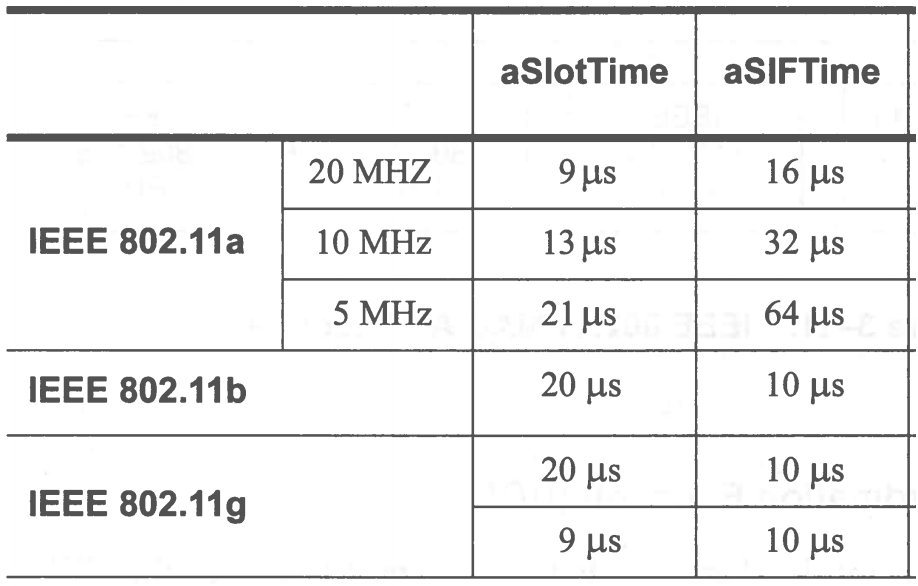
\includegraphics[width=14cm]{table-slot-time}
    \caption{Table showing different values of SIFS and Slot time for different PHY. Taken from \cite{Aboul-Magd2008WirelessPerspective}}
    \label{fig:table-st}
\end{figure}
% 
\begin{figure}
    \centering
    
\includegraphics[height=.95\textheight]{csma-ca}
    \caption{Flowchart showing the operation of CSMA/CA. The dotted square shows RTS/CTS protocol, implementation of which is voluntary. RTS/CTS is part of 802.11 standard. Source: \url{https://commons.wikimedia.org/wiki/File:Csma_ca.svg}}
    \label{fig:csma-ca}
\end{figure}
% 
As for performance of different standards, \cite{Bilgin2013PerformanceAreas} compares 802.11b with 802.11p. The authors compared these in various environments, various speeds and various packet sizes. Since testing this with multiple moving vehicles is very challenging, they used simulation software \emph{MOVE} to generate the movement of vehicles and \emph{NS-2} network simulator to evaluate the parameters of the wireless connection, such as throughput, packet delivery ratio and delay. 
Overall comprehensive analysis provided these results:\\ \textquote[\cite{Bilgin2013PerformanceAreas}]{\emph{Comparative performance evaluations show that IEEE 802.11p MAC layer protocol has better results for V2V communications compared to the IEEE 802.11b MAC protocol in terms of network throughput, end-to-end delay, and delivery ratio.}}\\
This conclusion should not be very surprising, as 802.11p was designed years after 802.11b specifically for use in vehicular environments. We will explore the 802.11p and its uses in the next section.

\subsubsection{802.11p} \label{sec:802.11p}
% 
802.11p is an amendment to standard 802.11 by \acrshort{IEEE}. This amendment was developed between 2005 and 2009 and was approved and published in 2010 as \enquote{Amendment 6: Wireless Access in Vehicular Environments}. It was included in 2012 revision of 802.11 and onwards.
802.11p is designed for \acrshort{V2V} and vehicle-to-infrastructure \acrshort{V2I} communication. This communication can often exist for short period of time only, therefore some of the properties (such as authentication) defined by original 802.11 standards are omitted. The 802.11p has served as base for the ITS-G5 standard (described in next section).\par
% 
% 
While 802.11b only introduced some changes in the \acrshort{PHY} layer to accommodate higher data rates in 2.4 GHz band, 802.11p introduces more significant changes in both \acrshort{PHY} and \acrshort{MAC} layers.
The \acrshort{PHY} characteristics of 802.11p are summed up in table \ref{table:11pPHY}.
% 
\begin{table}[h]
\centering
\begin{tabular}{|l|r|}
    \hline
    \rowcolor{lightgray} Specification & 802.11p \\
    \hline
    Data rate & 3, 4, 5, 6, 9, 12, 18, 24, 27 Mbps \\
    \hline
    Modulation & \acrshort{OFDM} \\
    \hline
    Coding rate & 1/2, 2/3, 3/4 \\
    \hline
    Number of subcarriers & 52 \\
    \hline
    \acrshort{OFDM} symbol duration & 8 $\upmu$s \\
    \hline
    Guard Time & 1.6 $\upmu$s \\
    \hline
    Preamble duration & 32 $\upmu$s \\
    \hline
    Subcarrier Spacing & 0.15625 MHz \\
    \hline
\end{tabular}
\caption{Specifications of 802.11p \acrshort{PHY} layer. Source: \cite{Abdelgader2014TheChallenges}}
\label{table:11pPHY}
\end{table}
% 
Some of the specifications are the same as for amendment 802.11a, to which 802.11p is often compared. The \acrshort{PHY} layer of 802.11p uses \acrshort{OFDM} modulation with 52 carriers.
They lie between 5,850–5,925 GHz (for the US) or 5,875–5,905 GHz (for Europe), which are frequencies licensed for vehicular use. The maximum range is 1000m in open space and maximum bandwidth is 27 Mbps \cite{Abdelgader2014TheChallenges}.
Out of those 52 carriers, 4 (\emph{pilot carriers}) are always transmitting the same pattern. This is used to correct possible phase and frequency offset on the receiver side (that may be present for example due to Doppler effect\footnotemark). The remaining 48 channels can be modulated using \acrshort{BPSK}, \acrshort{QPSK}, 16-\acrshort{QAM} or 64-\acrshort{QAM} modulation.\par
% 
\footnotetext{\textquote[Taken from: \url{https://en.wikipedia.org/wiki/Doppler_effect}, edited.]{\textit{The Doppler effect is the change in frequency or wavelength of a wave, for an observer moving relative to its source.}}}
% 
Compared to 802.11a, it has increased the guard time, just as well as symbol duration. These changes were made in order to account the problems arising from the high mobility scenarios (such as Doppler's effect).\par
% 
% \footnotetext{\url{http://www.rfwireless-world.com/Terminology/WLAN-802-11a-versus-802-11p.html}}
% 
The \acrshort{MAC} layer of 802.11p makes use of \emph{\acrfull{EDCA}}. This algorithm improves the DCF specified earlier by dividing traffic into 4 categories (so-called \emph{Access Classes - \acrshort{AC}s}):
% 
\begin{itemize}[noitemsep]
    \item background traffic (BK)
    \item best-effort traffic (BE)
    \item video traffic (VI)
    \item voice traffic (VO)
\end{itemize}
% 
Similarly to what was described in \hyperref[sec:802.11b]{802.11b}, \acrshort{CW} principle is used. The CVmax and CVmin values are specified in the standard, however, they vary for different \acrshort{AC}s. Furthermore, another parameter - \acrfull{AIFS} is defined for each of the \acrshort{AC}s. By combining \acrshort{CW} and \acrshort{AIFS} it is ensured, that more latency-sensitive content (such as voice call) will be sent sooner than not-latency-sensitive content (such as weather news).\par
% 
It has been argued \cite{Bilstrup2008EvaluationCommunication}, that vehicular use does not need different classes of content, and instead, a \emph{worst-case scenario channel access time} should be introduced. Simulations have shown, that 802.11p's \acrshort{DCF} (based on CSMA) is not very suitable for periodic broadcast messages (which are likely to be transmitted in an enhanced platooning scenario, where other vehicles need to be aware of the platoon's state.
% 
The main challenges in vehicular environment, often caused by high mobility of nodes, include signal fading, packet collisions and signal interference. The comparison of performance with 802.11b has been presented in previous section. Another possible solution for V2V communication is Japanese standard \acrshort{arib} T109 (described in following section). Performance-wise, \cite{Heinovski2016PerformanceSTD-T109} concludes, that \acrshort{arib} is more efficient in non-line of sight scenarios, which are often a case in urban environments. On the other hand, since \acrshort{arib} uses \acrshort{TDMA} (as opposed to CSMA in 802.11p), the transmission may be more delayed, as the node has to wait for next available time slot. In particular scenarios, 802.11p may be a better solution due to lower latency.\par
% 
Journal article \cite{HameedMir2014LTEEvaluation} compares 802.11p with \acrshort{LTE} network. \acrshort{LTE} is not considered in our report, however the paper brings in interesting insights. 802.11p is considered infrastructure-less standard, while \acrshort{LTE} requires significant infrastructure to operate. Though, simulations have shown, that \acrshort{LTE} performs better for most of the V2V related use-cases, due to better scheduling and channel access control.\par
\pagebreak

\subsubsection{\acrshort{wave}}
% 
\begin{center}
\textquote[\cite{VehicularTechnologySociety2014IEEEArchitecture}]{\emph{\acrshort{wave} protocols are designed to allow applications to exchange data in a consistent, interoperable, and timely manner.}}
\end{center}\par
% 
\acrfull{wave} is a set of comprising multiple standards, that aims for enabling \acrshort{V2V} and \acrshort{V2I} connectivity. Group of \acrshort{wave} standards includes extensions to the \acrshort{MAC} layer of 802.11 and several standards from the 1609 family. These standards specify the means of wireless communication on the four OSI model layers (physical, data link, network and transport layer). Furthermore, two standards specify the 'vertical' properties of the communication, such as security and remote management. Figure \ref{fig:wave-fam} shows part of the \acrshort{wave} set in detail, while Table \ref{tab:wave-stds} lists \acrshort{wave} standards and their use. The \acrshort{wave} family specifies certain frequency allocations and channels for the use in the US. While the frequencies could be adjusted for the use in other countries, standard bodies in Europe have developed own standard, thus we will skip certain details of how \acrshort{wave} works. European ITS-G5 is discussed \hyperref[sec:ITS-G5]{in the following section}.\par
% 
\begin{figure}
    \centering
    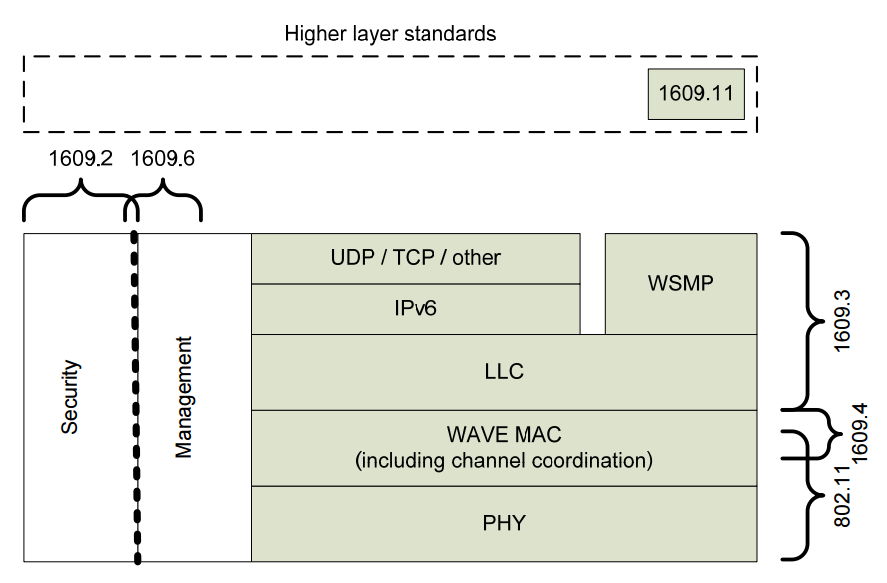
\includegraphics[width=.95\textwidth]{wave-fam}
    \caption{The standards of the \acrshort{wave} set shown together with the elements of the OSI model. Taken from \cite{VehicularTechnologySociety2014IEEEArchitecture}}
    \label{fig:wave-fam}
\end{figure}

\begin{sidewaystable}
    \centering
    \begin{tabular}{|p{5cm}|p{5cm}|p{9cm}|}
        \hline
         \textbf{IEEE Standard} & \textbf{Area} & \textbf{Features} \\
         \hline
         IEEE Std 1609.4-2010 & Extensions to IEEE 802.11 MAC layer. & 
         \begin{itemize}[nolistsep,noitemsep, topsep=0pt]
             \item Channel timing
             \item MAC addressing \& pseudo-anonymity
         \end{itemize} \\ \hline
        %  
         IEEE Std 1609.3-2010 & Networking Services & 
         \begin{itemize}[nolistsep,noitemsep, topsep=0pt]
             \item \acrshort{wave} service advertisement and channel scheduling
             \item \acrshort{wave} Short message protocol
         \end{itemize} \\ \hline
        %  
         IEEE Std 1609.2-2013 & Security Services for Applications and Management Messages &
         \begin{itemize}[nolistsep,noitemsep, topsep=0pt]
             \item Security for \acrshort{wave} Service Advertisements and \acrshort{wave} Short Messages
             \item Additional security services
         \end{itemize} \\ \hline
        %  
        IEEE Std 1609.11-2010 & Over-the-Air Electronic Payment Data Exchange Protocol for ITS & ISO-compliant payment protocol \\ \hline \hline
        %  
        \textbf{IEEE Project} & \textbf{Area} & \textbf{Features} \\ \hline
        % 
        IEEE P1609.6  & Remote Management Services & Over the air management and aliasing. \\ \hline
        % 
        IEEE P1609.5  & Communication Manager & Network management \\ \hline
    \end{tabular}
    \caption{Set of \acrshort{wave} standards and their respective areas. From \cite{VehicularTechnologySociety2014IEEEArchitecture}}.
    \label{tab:wave-stds}
\end{sidewaystable}
% 
As specified in \cite{VehicularTechnologySociety2014IEEEArchitecture}, \acrshort{wave} standards do not distinguish between types of devices connected. Instead, they are robust enough to accommodate communication to/from On-board Units (OBU), Road-side Units (RSU), together with portable units (e.g. smartphones) and pedestrian units (e.g. roadside workers). 
% 
\subsubsection*{Extensions of 802.11 MAC layer} 
The 802.11 standard and in particular its amendment - 802.11p, can be seen as the roots for the \acrshort{wave} family. 802.11p specifies the \acrshort{PHY} and \acrshort{MAC} layers of wireless communication suitable for vehicular environments. The newest revision of 1609.4 standard - \acrshort{IEEE} Std 1609.4-2016 specifies some additional features of the \acrshort{MAC} layer. It operates on frequency band 5.850GHz to 5.925GHz. While 0.005GHz at the lower edge is kept in reserve, the rest of the band is divided into 7 channels. These are further divided into \acrfull{CCH} and \acrfull{SCH}. Figure \ref{fig:wave-channels} describes channel allocation in detail.\par
% 
\begin{figure}[ht]
    \centering
    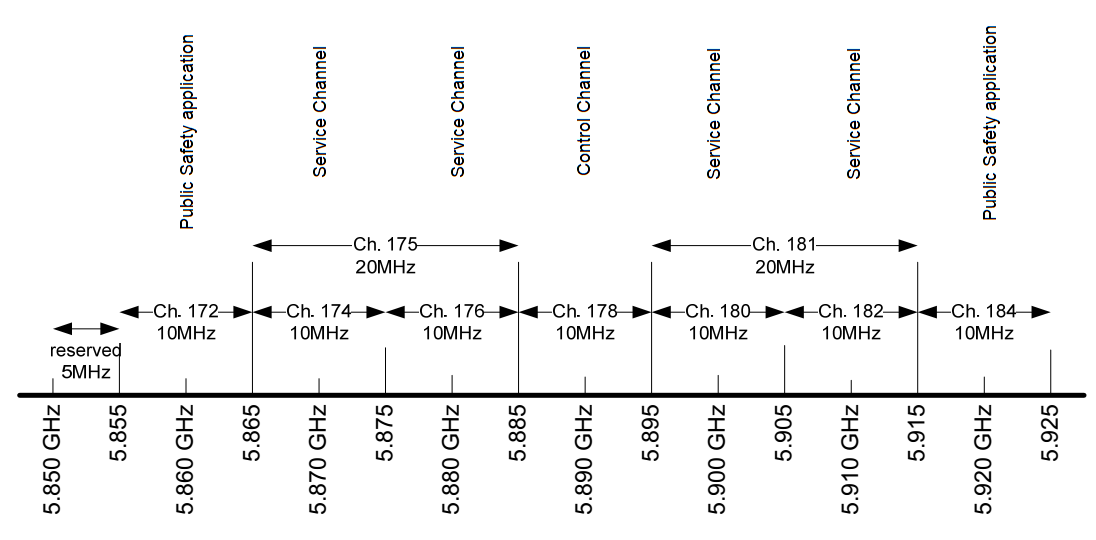
\includegraphics[width=.95\textwidth]{wave-channels}
    \caption{Figure showing channel frequencies and the use of the channels. Note that channels 174 and 176 and channels 180 and 182 can be merged to create channels 175 and 181 respectively. Taken from \cite[p. 20]{VehicularTechnologySociety2014IEEEArchitecture} (edited).}
    \label{fig:wave-channels}
\end{figure}
% 
The \acrshort{CCH} is reserved for system management messages and only allows communication via \acrfull{WSMP}. On \acrshort{SCH}, both \acrshort{IP} traffic (using IPv6 addresses) and \acrshort{WSMP} is possible. \acrshort{WSMP} is a protocol that sends \acrfull{WSM}, which are designed to consume minimal channel capacity. \acrshort{WSMP} allows transmitter device to specify physical characteristics of the transmission, such as transmitter power and channel used. The transmitter needs to provide MAC address of the receiver, however group MAC addresses are allowed. Furthermore, transmitter needs to provide a \acrfull{PSID}\footnotemark. The receiver can decide, based on the \acrshort{PSID} of received \acrshort{WSM}, if the message is of interest or should be discarded.\par
% 
\footnotetext{\textquote[\cite{20161609.12-2016Allocations}]{\acrshort{PSID} is an integer with a value from 0 to 270 549 119. [...] Each allocated \acrshort{PSID} value is associated with an organisation that is authorised to describe the use of that \acrshort{PSID}.}}
% 
A performance study comparing \acrshort{ETSI} ITS G5 and \acrshort{wave} \cite{Eckhoff2013AWAVE} suggests, that \acrshort{wave} is suitable for transmitting periodical Cooperative Awareness Messages. Those are likely the messages that would be used in platooning scenario. It may suffer from lower delivery rate and higher end-to-end delay in scenarios with high node densities and high penetration. This, however is the same for0\acrshort{ETSI} ITS G5, therefore we do not see these results as a major drawback of \acrshort{wave}. Overall, we can conclude that \acrshort{wave} is ready to facilitate platooning. After all - \emph{Vehicle communication for collision avoidance}, which shares some of the characteristics with platooning (like Forward collision warning, Longitudinal collision risk warning) and would likely need similar type of communication architecture as platooning, is a representative use case in \acrshort{IEEE} Guide for \acrshort{wave} architecture (\cite{VehicularTechnologySociety2014IEEEArchitecture}).

\subsubsection{ETSI ITS-G5}\label{sec:ITS-G5}
% http://www.etsi.org/deliver/etsi_en/302600_302699/302663/01.02.00_20/en_302663v010200a.pdf
ITS-G5 is a Dedicated Short Range Communication (DSRC) standard, running on the 5GHz frequency band based on \hyperref[sec:802.11p]{802.11p} in Europe.
The spectrum allocated for DSRC is 5.875-5.905 GHz also called ITS-G5A. This allocated spectrum of 30 MHz is only for ITS. Of the 30 MHz only a third of that is saved for the Road safety as seen on the picture below.\par
% 
The protocol stack for ETSI ITS G5 uses IEEE 802.11p as the physical layer. By dividing channels into Control Channel (CCH) and Service Channel (SCH), packets transmit through the control channel do not have to compete with service channel. For Medium access layer, channel access and priority is done by Enhanced Distributed Channel Access (EDCA) by using a variation of CSMA/CA. The packets not only compete for channel access with other vehicles but also with packets internally in the same node. Packets are divided by 4 access categories, VO, VI, BE and BK. Each access categories can be given one of the two channel types, resulting in 8 different combinations. Internal congestion control is being done (one for CCH and one for SCH) before the packet is sent to their respective queue. ETSI ITS G5 also performs a Decentralised Congestion Control (DCC), which changes transmit power, the minimum packet interval, the data rate, and the sensitivity of the radio accordingly. It does this by acting like a state machine going from a “active”, “relaxed” and “restrictive” state depending on the situation.
ETSI ITS G5 periodically transmit broadcast message called CAMs with information about their current state, location, speed, and direction with a frequency of 10 Hz.\par
% 
As described in conference proceedings for IEEE 79th Vehicular Technology Conference: \textquote[\cite{Shi2014SpectrumSafety}]{\textit{We performed extensive simulation for CSMA/CA and STDMA MAC (Simulation parameters) schemes in an urban highway scenario with realistic traffic density. Results show that more than 80 MHz is required to achieve 1\% packet loss with 500 m communication range. It is significantly larger than the current spectrum allocated of 10 MHz in the US and Europe.}}\par 
% 
It is also mentioned that by decreasing the communication range to 100 m, the spectrum requirement is reduced to 20 MHz, still being twice the amount available today. 

\subsubsection{ARIB STD-T109}
% 
% Section about Japanese technology ARIB.
ARIB STD-T109 is a standard developed by Association of Radio Industries and Businesses, a Japanese-based organisation. The standard was developed to \textquote[\cite{2012ARIB1.0}]{\textit{Enable effective use of radio frequencies by avoiding interference among users}}, for use in intelligent transportation systems.\par
% 
The radio communication requirements for ARIB (Association of Radio Industries and Businesses) consist of single channel radio communication in the 700 MHz band with both V2I and V2V communication. The communication have to support V2V communication up to 140 km/h and V2I up to 70 km/h.\par
% 
The protocol stack of ARIB STD-t109 is of a 4 layer-structure.
Layer 1: Physical layer. It consist of 2 sublayers, physical medium dependent (PMD) sublayer and physical layer convergence protocol (PLCP) sublayer. The PMD sublayer gives a method to transmit and receive data between stations (V2I or V2V) that uses OFDM (Orthogonal frequency-division multiplexing).
Layer 2: Data link layer. It consist of 2 sublayers, MAC sublayer and LLC (Logical Link ontrol) sublayer. In the MAC sublayer CSMA/CA (Carrier sense multiple access / collision avoidance) is used for multiple access control method. The LLC sublayer lets unacknowledged services (data without error control and no guarantee of delivery) to transmit packets between upper layers.
V2V\&V2I layer: Inter-vehicle and Roadside-to-vehicle communication layer. It creates and manages data required for V2I and V2V communication control. It also makes a method to give parameters needed for communication control for the MAC sublayer (synchronises clocks etc).
Layer 7: Application layer. It gives a communication control method and services for applications such as security and it also gives a method to transmit and receive data through the V2V\&V2I layer. 
\par
The protocol data unit (PDU) of the MAC and LLC sublayer can be seen on the picture below.
\begin{figure}
    \centering
    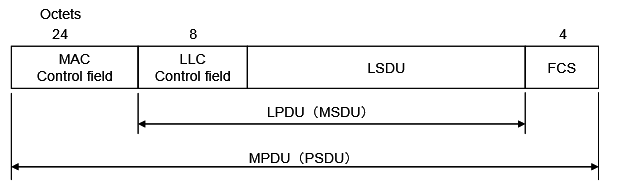
\includegraphics[width=14cm]{PSDU}
    \caption{Shows MAC protocol in parts}
    \label{fig:PSDU}
\end{figure}

A PDU of MAC called MAC protocol data unit (MPDU) consists of 4 elements. MAC Control field, LLC control field, Link service data unit (LSDU) and frame check sequence (FCS).
MAC control field's length is 24 octet and contain information needed to control and establishing connection, it can be broken down to 6 fields with each of their length shown below.
\begin{figure}
    \centering
    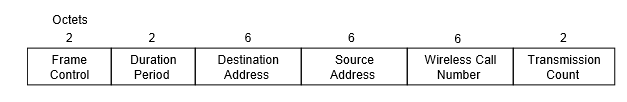
\includegraphics[width=14cm]{MAC}
    \caption{Shows breakdown of MAC Control field}
    \label{fig:MAC}
\end{figure}


Frame control has the data for what type of frames and fields is coming up. Duration period contains duration value for each frame. Destination Address is the receiver's MAC address. Source Address is the senders MAC address. Wireless call number is a identification code for security reasons. Transmission count is a number which goes up by 1 for each transmission. 

LLC control field can be split into 4 fields. DSAP address field identifies which Service Access points (SAPs) is intended for the LLC PDU. SSAP Address field identifies if the LLC PDU is a command or response PDU. Control field contains command, response, and sequence number information. Protocol identifier field sees if the right protocol is being used.
\begin{figure}[h]
    \centering
    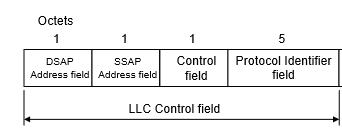
\includegraphics[width=14cm]{LLC-control-field}
    \caption{Shows breakdown of LLC control field}
    \label{fig:LLC}
\end{figure}
Lastly is the Link service data unit and Frame check sequence, which helps detect data errors that might have happened during the transmission, by checking if the number based on the data matches the FCS number, after receiving the data. 
\par
% 
Though ARIB is using the same physical layer as IEEE 802.11, one of the key differences is that the MAC address not only is being used to identify which service access point (SAPs) of the layers but also to distinguish between communication traffic between V2V and V2I. The TDMA (Time-division multiple access) scheme is used by having control cycles of 100.000$\upmu$s which is then divided into 16 smaller cycles of  6240$\upmu$s. Each of the small cycles have 2 periods, the first period, 0 to 3024$\upmu$s is called V2I period which is the period where only that form of communication access is allowed in the channel. The reason is that the infrastructure is connected to multiple sensors scattered around the road, giving it more knowledge about the current situation than a vehicle for distributing safety information. Since each infrastructure can be allocated a specific time-slot in the V2I period, it is not necessary to use CSMA/CA. After the V2I period ends (after 3024$\upmu$s), vehicles can compete for channel access, but to avoid concurrent channel access with other vehicles, CSMA/CA is used \cite{Heinovski2016PerformanceSTD-T109}.\par
% 
Like the IEEE 802.11 and ETSI, ARIB also uses OFDM (Orthogonal Frequency Division 
Multiplexing) as modulation scheme. OFDM uses BPSK, QPSK, 16-QAM and 64-QAM\footnotemark.\par
% 
\footnotetext{\url{http://rfmw.em.keysight.com/wireless/helpfiles/n7617a/coding_and_modulation.htm}, accessed on 17/04/2017}
% 
ARIB using both TDMA and CSMA/CA (compare to 802.11p only using CSMA/CA) gives it a better communication distance in urban environment almost up to 3 times the distance \cite{Heinovski2016PerformanceSTD-T109}, because it suffers less from obstacles such as buildings etc. On the other hand, because of the priority of the V2I period, it causes packet losses for the traffic between vehicles. For same reason, message delays also happen, since they need to wait for the next time slot, which is not reserved, and this causes delay. 

\subsection{GPS}
One of the important information needed for platooning, is the ability to know the exact location of a car or any vehicle in the VANET system. By taking advantage of the Global Positioning System (GPS) it is possible to do so.\par
% 
% 
The GPS work by having at least 24 satellites orbiting the earth, ground stations and lastly a receiver. 4 visible satellites sends out microwave signals to the receiver, which then uses triangulation to figure out where the receiver is on earth. Though only 3 satellites are needed for the triangulation, the 4th is a safety measure in case the calculation is wrong or if altitude and latitude is needed. The ground stations is to know where the satellites are in relative to the earth \cite{MiTACIntl.2011HowWork}.\par
% 
% 
Every microwave is sent on exact intervals, the data in the signal is the ID of the satellite, the location of all the satellites and time. With this information, the receiver can do the trilateration process and determine the location of the receiver.

\subsection{Conclusion}

We can see that authorities are aware of the need for inter-vehicular communication. Developed standards and allocated frequency bands indicate the readiness for the platooning scenario. Although the standards are still very recent and it may take a while, before all the issues are resolved (e.g. quality of service issues during higher node penetration in \acrshort{wave} \& \acrshort{ETSI} ITS-G5), generally, there is technology capable of transmitting any data required for the platooning to be enabled. There are some differences among regions of world, for instance the \acrshort{arib} vs. 802.11p standards, which use different protocols and different frequencies. These differences, however are mostly present on the \acrshort{PHY} and \acrshort{MAC} layer, thus a uniform solution can be developed on the higher layers, if 802.11p, ITS-G5 or \acrshort{arib} is used. \acrshort{wave} architecture even contains standards and guidelines for the communication at network and transport layer, thus allowing for even easier adoption of platooning.
\pagebreak

\section{Analysis}\label{sec:Analysis}

//Analysis goes here\par
% 
\subsection{Motivation}

Companies internally can easily manage to arrange platooning by scheduling time and routes accordingly, to match with other deliveries. This can be done by having multiple trucks go from A to B on the same time or having their starting point in different location and then meet up at an intersection. Since it is inside the company, making the drivers use the platooning system to save fuel is a possible requirement to force on the drivers. This would lead to the company saving money through usage of fuel (ref) on the cost of more logistic and initial cost of platooning technology.\par
% 
This is slightly harder to do when it comes across different companies. The temporary solution could be that companies have a partnership, giving them the information needed to arrange their routes together to form platooning. This solution would be the same as the internal company, since it would be like 1 big company working together. Since the front truck uses more fuel than the later trucks, an agreement in the contract to share the fuel consumption would have to be made in the partnership. This however would only be a temporary solution since partnership would not be possible to do with everyone, and new upstarting companies or smaller companies would not be able to join in those partnerships to begin with.\par
% 
To take it one step further and remove the partnership and let anyone with the technology and wants to be in a platooning can do so. While internal companies can keep doing their platooning as usual, other nearby trucks can join the platoon on the cost of a small fee to the front truck for each km driven together in the platoon. This would be a solution where everyone benefits, since the initial company who started the platooning is saving even more fuel with the addition of the new truck giving them extra money from the fee. If another truck joins the platoon, the 2nd last truck pays a slightly higher fee than before (since their fuel consumption is the lowest of them all) and the last truck pays a small fee as usual. By giving a small fee to the fist truck, it will not discourage truck drivers to be the frontal truck and no matter where you are in the platoon you will always save money, even when being the last.
(picture that explains the situation maybe?)
% 
\subsection{Control WIP title etc etc}
Projects have given the truck drivers different level of control while platooning. Some had the front truck driver driving the truck manually or with a speed controller, while the following trucks only needed to steer, and having the speed and break be controlled by the computer. Others had speed, break steering being taken over by the computer. Both cases had a driver ready to take over in case something would go wrong and is in need of a overwriting of the truck driver.\par
% 
\par
< something > 
\par
% 
Around 94 percentage of car crashes in the US (2015) is estimated to be the result of the driver. This can be drastically reduced by having autonomous driver, meaning, giving the driver as little control as possible. This is on paper a good thing, but is a completely different thing in reality. As most things that concerns safety of human life, when new technology appears, many are in distrust regarding it. A statistic shows that in US and UK there is as little as 15 percentage who are not concerned with this technology at all, while 26 percentage is very concerned in the US. 

\pagebreak

\section{Discussion}

//Discussion goes here
\pagebreak

\section{Conclusion}\label{sec:conclusion}
%
To solve a problem of congestion, safety and fuel consumption different technologies and models have been and are being developed. Platooning is one of them, which by making use of \acrshort{V2V} and \acrshort{V2I} communication and additional infrastructure (such as radars, sensors, etc.) enables vehicles to drive at close distances autonomously by following the leading vehicle with a driver. We liked this idea and therefore we decided to dig into it and try to find some solution for platooning.\par
%
Our aim was to research platooning and propose a possible solution for it, which would satisfy the requirements proposed in \hyperref[sec:requirements]{\textit{Requirement specification} chapter}. These requirements were based on \hyperref[sec:stakeholders]{\textit{Stakeholder analysis}}, secondary data and interviews. Not all requirements were successfully met because we have not been developing whole system for platooning, we are only suggesting a possible solution for ad hoc platooning communication. It should also be tested theoretically and practically. However, the technologies chosen in \hyperref[sec:analysis]{\textit{Analysis} chapter} were chosen in a way that they all can safely meet requirements.\par
%
At the beginning of research about technology and collection of secondary data, we contacted several of our possible stakeholders (Scania, Car2car communication consortium, Danish road authority, Danish transport organisation for drivers), kindly asking them for an interview. Unfortunately, we only got one response - from Danish transport organisation for drivers from which we got a contact - truck test driver who has been testing platooning. We did an interview with him and findings were interpreted in \hyperref[sec:data]{\textit{Empirical data} chapter}.\par
%
While the research about platooning is still ongoing, we investigated projects and researches that has been finished recently. We were surprised that platooning is not just something from this era, but the idea dates back to the 20th century. The most interesting and relevant projects such as SARTRE \cite{Chan2012ProjectSARTRE}, Companion \cite{2016CompanionProject} or Safespot \cite{Safespot}, were picked and analysed thoroughly to get inspiration, insights and secondary data. These and a few more were then processed in the \hyperref[sec:literature]{\textit{Literature review} chapter}.\par
%
Reading and analysing existing project was not enough to gather all needed data about the topic. In \hyperref[sec:technology]{\textit{Technology} chapter}, various technologies were analysed in order to answer the problem formulation better. Therefore, more research had to be conducted, in the field of technology. The \acrshort{V2V}, \acrshort{V2I} and \acrshort{VANET} were studied in order to understand these principles better. To find the right technology for platooning existing and emerging technologies such as 802.11p, ITS-G5, \acrshort{wave} or \acrshort{arib} STD-T109 were analysed with their potential use and benefits. \par
%
Having all the necessary areas researched giving us a lot of information, there was only one last thing needed - analyse material and propose a solution. This is done in \hyperref[sec:analysis]{\textit{Analysis} chapter}. There motivation section explains why freight companies should be interested in platooning and what the motivation for them may be. Then an architecture of the overall system is proposed. A few architectures are discussed there with their strengths and weaknesses presented. Technology section in Analysis shows possible technologies fulfilling our requirements. We found out that all of the researched technologies does that and therefore can be used for platooning, though each of them has their pros and cons. The last part of Analysis shows advantages of autonomous systems which are in favour in platooning overally while attitude of people is not. \par
% 
\vspace{2cm}
%
% 
\cite{Caldwell1999TwoWave}
% 

\begin{picture}(20,200)
    \put(0,120){\hbox{
\includegraphics[scale=0.8]{00000}}}
\end{picture}
\pagebreak

\printbibliography[heading=bibintoc]
\pagebreak

\appendix
\section{Appendix - Interview guide for a Platoon test driver}

This interview guide contains wide spectrum of questions regarding truck platooning and platooning in general. Interviewee is a platoon test driver, which is very fortunate for our research reasons. We are concentrating on higher level platoon architecture and communication, meaning all participants of V2V and V2I communication, although insights from potential user(driver) who already has experience with platooning might give us different angle to look at the problem.\par
% 
General questions about platooning and its implementation:
\begin{itemize}[noitemsep]
    \item Please tell us about research/development you are part of. What are the goals of whole study?
    \item How does the setup/architecture of platoon in your case looks like? Fully or partial automated? How many trucks (minimum-maximum numbers)?
    \item What limitations/requirements does your project contains? Only highways? EU roads or worldwide? 
    \item What are the reasons of those limitations/requirements? Technology? Law? People are not ready to accept platooning?
    \item As an inside man maybe you can predict when and to what level platooning will be implemented on the roads? \\
    %
    \item As a test driver please elaborate on what are critical and maybe unexpected findings after researching and testing platooning on the roads?
    \item What advantages and disadvantages platooning brings to truck drivers? Do drivers feel positively about upcoming technologies?
\end{itemize}
%
\par
%
More in depth technical questions:
\begin{itemize}[noitemsep]
    \item What kinds of communication your project includes? V2V, V2I? Is it dependant on road infrastructure?
    \item What types of technologies are used for V2V? Why?
    \item What are the main concerns regarding vehicle to vehicle communication?
    \item What types of technologies used for V2I (if used)? Why?
    \item Main concerns for vehicle to infrastructure communication?
\end{itemize}

\end{document}
